%----------------------------------------------------------------------------------------
% 	Template: Abschlussarbeiten des Studiengangs Angewandte Informatik an der HTW Berlin
% 	C. Schmidt 
%----------------------------------------------------------------------------------------
%	Pakete und Konfigurationen
%----------------------------------------------------------------------------------------
%\documentclass[twoside,twocolumn]{article}
%\documentclass[german,a4paper,12pt,oneside]{scrbook}
\documentclass[oneside,bibliography=totocnumbered,BCOR=5mm]{scrbook}% Voreinstellungen entfernt.

%\usepackage[latin1]{inputenc}
\usepackage{amsmath, amsthm, amssymb}
%\usepackage[ngerman]{babel} 
\usepackage[utf8]{inputenc}
\usepackage{array}
%\usepackage[english]{babel} % Language hyphenation and typographical rules
%\usepackage{marvosym}
%\usepackage{scrhack}
\usepackage{graphicx}
%\usepackage{graphics}
\usepackage{csquotes}
\newtheorem{satz}{Satz}[chapter]
\theoremstyle{definition} 
\newtheorem{definition}[satz]{Definition} 
\theoremstyle{definition} 
\newtheorem{lemma}[satz]{Lemma} 
\theoremstyle{definition} 
\newtheorem{bemerkung}[satz]{Bemerkung}
\theoremstyle{definition} 
\newtheorem{korollar}[satz]{Korollar} 
\theoremstyle{definition}
\newtheorem{beispiel}[satz]{Beispiel} 
\theoremstyle{definition} 
\newtheorem{algorithmus}{Algorithmus} 
\newenvironment{beweis}{\begin{proof}[Beweis]}{\end{proof}}
\usepackage[hyphens]{url}
\usepackage{hyperref}

%----------------------------------------------------------------------------------------
%	BIB.-Datei und Quellenverwaltung
%----------------------------------------------------------------------------------------
\usepackage[backend=bibtex, style=numeric]{biblatex}
\addbibresource{thesis.bib}
%----------------------------------------------------------------------------------------
\usepackage{blindtext} % Package to generate dummy text throughout this template 

\usepackage[sc]{mathpazo} % Use the Palatino font
\usepackage[T1]{fontenc} % Use 8-bit encoding that has 256 glyphs
\linespread{1.05} % Line spacing - Palatino needs more space between lines
\usepackage{microtype} % Slightly tweak font spacing for aesthetics

\usepackage[hmarginratio=1:1,top=32mm,columnsep=20pt]{geometry} % Document margins
\usepackage[hang, small,labelfont=bf,up,textfont=it,up]{caption} % Custom captions under/above floats in tables or figures
\usepackage{booktabs} % Horizontal rules in tables
\usepackage{lettrine} % The lettrine is the first enlarged letter at the beginning of the text
\usepackage{enumitem} % Customized lists
\setlist[itemize]{noitemsep} % Make itemize lists more compact

\usepackage{titling} % Customizing the title section

%----------------------------------------------------------------------------------------
%	Listings
%----------------------------------------------------------------------------------------
\usepackage{listings}
\usepackage{color}

\usepackage{lmodern}
\definecolor{mygreen}{rgb}{0,0.6,0}
\definecolor{mygray}{rgb}{0.5,0.5,0.5}
\definecolor{mymauve}{rgb}{0.58,0,0.82}

\lstset{ 
  backgroundcolor=\color{white},   % choose the background color; you must add \usepackage{color} or \usepackage{xcolor}; should come as last argument
  basicstyle=\footnotesize,        % the size of the fonts that are used for the code
  breakatwhitespace=false,         % sets if automatic breaks should only happen at whitespace
  breaklines=true,                 % sets automatic line breaking
  captionpos=b,                    % sets the caption-position to bottom
  commentstyle=\color{mygreen},    % comment style
  deletekeywords={...},            % if you want to delete keywords from the given language
  escapeinside={\%*}{*)},          % if you want to add LaTeX within your code
  extendedchars=true,              % lets you use non-ASCII characters; for 8-bits encodings only, does not work with UTF-8
  firstnumber=1,                % start line enumeration with line 1000
  frame=single,	                   % adds a frame around the code
  keepspaces=true,                 % keeps spaces in text, useful for keeping indentation of code (possibly needs columns=flexible)
  keywordstyle=\color{blue},       % keyword style
  language=Octave,                 % the language of the code
  morekeywords={*,...},            % if you want to add more keywords to the set
  numbers=left,                    % where to put the line-numbers; possible values are (none, left, right)
  numbersep=5pt,                   % how far the line-numbers are from the code
  numberstyle=\tiny\color{mygray}, % the style that is used for the line-numbers
  rulecolor=\color{black},         % if not set, the frame-color may be changed on line-breaks within not-black text (e.g. comments (green here))
  showspaces=false,                % show spaces everywhere adding particular underscores; it overrides 'showstringspaces'
  showstringspaces=false,          % underline spaces within strings only
  showtabs=false,                  % show tabs within strings adding particular underscores
  stepnumber=1,                    % the step between two line-numbers. If it's 1, each line will be numbered
  stringstyle=\color{mymauve},     % string literal style
  tabsize=2,	                   % sets default tabsize to 2 spaces
  title=\lstname                   % show the filename of files included with \lstinputlisting; also try caption instead of title
}


\newenvironment{conditions}[1][mit:]
  {#1 \begin{tabular}[t]{>{$}l<{$} @{${}={}$} l}}
  {\end{tabular}\\[\belowdisplayskip]}

%----------------------------------------------------------------------------------------
%	Haupttextteil
%----------------------------------------------------------------------------------------

\begin{document}
% Titelseite
% \pagestyle{empty}       % keine Seitennummer
\begin{titlepage}
\begin{center}

\includegraphics{images/HTW_Berlin_Logo_farbig.jpg}
\linebreak[4]
\linebreak[4]
\linebreak[4]
\linebreak[4]
\textit{\large Erkennung und Korrektur von Sequenzierungsfehlern in DNA-Sequenzen}
\linebreak[4]
\linebreak[4]
\linebreak[4]
Abschlussarbeit 
\linebreak[4]
\linebreak[4]
zur Erlangung des akademischen Grades: 
\linebreak[4]
\linebreak[4]
\textbf{Bachelor of Science (B.Sc.)} 
\linebreak[4]
\linebreak[4]
an der
\linebreak[4]
\linebreak[4]
Hochschule für Technik und Wirtschaft (HTW) Berlin
\linebreak[4]
Fachbereich 4: Informatik, Kommunikation und Wirtschaft
\linebreak[4]
Studiengang \textit{Angewandte Informatik}
\linebreak[4]
\linebreak[4]
\linebreak[4]
1. Gutachter\_in: Herr Prof. Dr. Christian Herta\linebreak[4]
2. Gutachter\_in: Herr Dr. Christian Krumnow\linebreak[4]
\linebreak[4]
\linebreak[4]
\linebreak[4]
\linebreak[4]
Eingereicht von Fabian Vogt [Matrikelnr. s0570800]
\linebreak[4]
\linebreak[4]
\linebreak[4]
\linebreak[4]
10.12.2022

\end{center}
\end{titlepage}
\newpage    % Seitenwechsel

\thispagestyle{empty}       % keine Seitennummer
% vertikaler Leerraum
\vspace*{2.2cm}
\noindent %kein Einzug
{\Huge Danksagung}\\
\vspace*{1.6cm} \\

% Kopfzeilen (automatisch erzeugt)
%\pagestyle{headings}
[Text der Danksagung]

% Seite mit Abstracts
\newpage
\thispagestyle{empty}    

\section*{Abstract}
Fehler beim Einlesen beziehungsweise Sequenzieren von DNA-Strängen können schwerwiegende Auswirkungen haben und sind daher von großer Bedeutung für die Genomanalyse. 
Sie können dazu führen, dass wichtige Informationen verloren gehen oder dass falsche Ergebnisse produziert werden, die zu falschen Schlussfolgerungen führen können. 
In der biomedizinischen Forschung können Sequenzierungsfehler zu inkorrekten Erkenntnissen führen, die wiederum in fehlerhaften Behandlungen resultieren können. 
Auch in anderen Bereichen, in denen DNA-Sequenzen analysiert werden, wie zum Beispiel in der Landwirtschaft oder in der Industrie, 
können diese Fehler zu Problemen führen.

Es gibt verschiedene Ansätze, wie mit Sequenzierungsfehlern umgegangen werden kann.
Eine Möglichkeit ist die Verwendung von Algorithmen, die speziell dafür entwickelt wurden, 
Fehler in DNA-Sequenzen zu erkennen und zu korrigieren. 
Diese Algorithmen funktionieren beispielsweise, indem sie bekannte Muster oder Merkmale in der DNA suchen, 
die auf Fehler hinweisen, oder indem sie die DNA-Sequenz mit bekannten, 
fehlerfreien Sequenzen vergleichen um Abweichungen zu erkennen. 

Es gibt auch verschiedene Qualitätskontrollmethoden, die verwendet werden können, um Fehler in DNA-Sequenzen zu minimieren, 
zum Beispiel durch Wiederholung von Messungen oder durch die Verwendung von redundanten Technologien.

Es ist wichtig, die geeignete Methode für das spezifische Anwendungsgebiet auszuwählen. 
Diese Wahl hängt von verschiedenen Faktoren ab, wie dem Fehlertyp, dem Fehlerrate und der gewünschten Genauigkeit der Analyse.

In dieser Bachelorarbeit werden verschiedene Methoden des Reinforcement Learning 
zur Erkennung und Korrektur von Sequenzierungsfehlern untersucht und miteinander verglichen. 
Die Stärken und Schwächen der Methoden werden analysiert und die geeignetsten Ansätze für verschiedene Anwendungsszenarien werden empfohlen. 
Durch die Überprüfung verschiedener Techniken und die Empfehlung geeigneter Ansätze soll diese Arbeit dazu beitragen, 
das Verständnis für die Korrektur von Sequenzierungsfehlern in DNA-Sequenzen zu verbessern. 
Insbesondere soll die Fehlererkennung und -korrektur durch Reinforcement Learning als Ansatz 
untersucht, bewertet und mit anderen Methoden des Maschinellen Lernens verglichen werden.



\clearpage
%Seite 1
\pagenumbering{roman}% Seitennummerierung "roemisch"
%\setcounter{page}{1} 

\tableofcontents  


%Seite 

 \listoffigures
 
 %Seite 6

 \listoftables
 


 \lstlistoflistings

.

\newpage

\pagenumbering{arabic}  % Nummerierung der Seiten in 'arabisch' % neues Kapitel mit Namen "Introduction"
 %Seite 1
 % \setcounter{page}{1}   % setzt Seitenzaehlung auf 1


\chapter{Einleitung}
\section{Motivation}
Die Korrektur von Sequenzierungsfehlern in DNA ist von entscheidener Wichtigkeit bei der Analyse von DNA
und der Diagnose und Behandlung von Krankheiten, die auf Ergebnisse der DNA-Untersuchung zurückzuführen sind.


Bei der DNA-Sequenzierung entstehen Fehler mit einer bestimmten Wahrscheinlichkeit, die von der Art des verwendeten Sequenzierungsverfahren abhängt.
Wenn beim Einlesen einer einzelnen Base ein Fehler passiert, wird diese mit einer anderen Base verwechselt.


Oft haben Sequenzierungsfehler nur wenig Einfluss auf eine Diagnose, da die DNA mehrfach gelesen wird und Fehler dadurch
zum Teil ausgeschlossen werden können.
Wenn aus einem fehlerhaften DNA-Read jedoch eine Fehldiagnose entsteht, können die Konsequenzen verherrend sein. 


Daher ist es wichtig, dass Sequenzierungsfehler korrigiert werden. 
Entweder muss ein Fehler direkt korrigierbar sein, oder er muss wenigstens erkannt werden, 
sodass der fehlerhafte Teil der Sequenz noch einmal eingelesen werden kann. 


\section{Problem- und Zielstellung (Scope)}
Es wird untersucht, ob fehlerhafte DNA-Sequenzen mit Hilfe eines Reinforcement-Learning Algorithmus korrigiert werden können. 
Das Problem wird modeliert, indem unverfälschte, menschliche DNA-Reads künstlich verfälscht werden. 
Daraus entsteht ein Trainingsdatensatz aus fehlerhaften DNA-Sequenzen und ihren jeweils unverfälschten Originalen.
Dieser Trainingsdatensatz wird genutzt, um Reinforcement-Learning Agenten zu trainieren.


Anstatt die fehlerhafte DNA-Sequenz direkt als Input zu nutzen, wird das DNABERT Transformer Model genutzt um eine 
kodierte Repräsentation der Sequenz zu generieren. 
DNABERT wurde unter anderem darauf trainiert, unbekannte (maskierte) Basen in DNA-Sequenzen zu bestimmen. 
Dadurch besitzt das Model ein gewisses Verständnis der Sprache der DNA, 
welches als abstrakter Vektor in den Hidden-States des Models kodiert ist. 
DNABERT verarbeitet die Sequenz Base für Base, somit wird für jede Base ein Hidden-State berechnet,
welcher sowohl Informationen über die aktuelle Base als auch über den Rest der Sequenz enthält.
Es ist die kodierte Repräsentation der jeweiligen Base im Kontext der Gesamtsequenz.
In der Theorie könnte ein einziger Hidden-State bereits genug Informationen enthalten, 
um entscheiden zu können ob dahinter eine fehlerhafte Base steckt.


Durch Verwendung der DNABERT-Hidden-States, anstelle einer simpleren, selbstgewählten Kodierung einzelner Basen, 
soll der Reinforcement-Learning-Agent schneller in der Lage sein, die fehlerhaften Basen zu erkennen. 
Die Informationen über die Syntax der DNA-Sprache sind bereits im Input-State vorhanden, 
dadurch wird das Problem im Idealfall auf ein reines Klassifikationsproblem reduziert. 
Wäre dies nicht der Fall, so müsste der RL-Agent zunächst die Sprache der DNA erlernen, 
um anschließend eine komplett eigenständige Entscheidung für die Bewertung einer Base 
im Bezug auf die Gesamtsequenz treffen zu können.


Die Fehlererkennung und Korrektur soll in verschiedenen Umgebungen mit unterschiedlichen Ansätzen
getestet werden. Dabei wird unterschieden zwischen reiner Fehlererkennung, ohne bestimmung der
korrekten Base, und Fehlerkorrektur mit bestimmung der Base. Für die Fehlerkorrektur wird zusätzlich
zunterschieden zwischen einer eigenständigen Korrektur durch den Reinforcement-Learning-Agenten und 
der Korrektur mit Hilfe der Maskierungsfunktion des DNABERT.
Außerdem wird getestet, ob das Training des Agenten mit besser funktioniert, wenn er die Sequenz als ganzes verarbeitet,
oder ob eine Basenweise Verarbeitung besser geeignet ist.


Als Ergebnis sollen Testergebnisse für Modelle vorliegen, die in den genannten Umgebungen trainiert wurden.
Außerdem soll eine Beurteilung entstehen, ob und wie weit sich ein Reinforcement-Learning-Ansatz 
zur Lösung des Problems eignet.



\section{Aufbau der Arbeit}


Am Anfang der Arbeit werden die theoretischen Hintergründe erläutert. 
Zuerst wird ein Überblick über das Thema DNA-Sequenzierung gegeben.
Was ist DNA-Sequenzierung und wofür wird es verwendet?
Was sind die gängigsten Sequenzierungsverfahren?
Wie können dabei Fehler entstehen?
Was sind mögliche Ansätze, um Sequenzierungsfehler zu korrigieren?
Außerdem wird erläutert, warum DNA einer Art von Sprache gleicht und 
somit der Bezug zum Thema Natural Language Processing (NLP) hergestellt.
Im folgenden werden das Transfomer- und das BERT-Model erläutert, welche eine wichtige Bedeutung 
für den Bereich NLP haben.
Zudem wird auch das DNABERT-Model vorgestellt, welches eine Weiterenticklung des BERT-Models ist 
und als Grundlage für Fehlerkorrektur durch einen Reinforcement Learning Agenten gilt.
Um den theoretischen Teil der Arbeit abzuschließen, werden das grundlegende Konzept des 
Reinforcement Learning und die verschienden Ansätze für die Fehlererkennung erklärt.


Die zweite Hälfte der Arbeit befasst sich mit der Implementierung des Reinforcement Learning.
Es werden die genutzten Frameworks gezeigt und erklärt, weshalb diese verwendet wurden.
Zwei grundlegend verschiedene Ansätze werden miteinander verglichen, Die Fehlererkennung und die Fehlerkorrektur.
Außerdem wird erläutert, wie die Belohnung des RL-Agenten berechnet wird. 


Zum Schluss folgt ein Fazit, in dem bewertet wird, wie gut sich die Verwendung von Reinforcement-Learning 
als Ansatz für die Fehlerkorrekturvon DNA-Sequenzen eignet.


Diese Arbeit trägt somit zum Verständnis bei, ob und wie Reinforcement Learning angewendet werden kann um die Fehlerkorrektur in 
DNA-Sequenzen zu verbessern und versucht somit eine höhere Genauigkeit in der Genomforschung zu erzielen.


\chapter{Theoretische Grundlagen}

\section{Kontext}

Die Arbeit hat einen molekularbiologischen Kontext, speziell die Sequenzierung von DNA-Strängen, 
wie dabei Fehler entstehen können und was mögliche Ansätze sind, diese Fehler zu korrigieren.
DNA-Sequenzierung hat die medizinische Forschung grundlegend verändert und neue, bessere Therapiechancen eröffnet. 
Die verwendeten Sequenzierungsverfahren wurden mit der Zeit optimiert und ihre Fehlerrate wurde stark reduziert. 
Trotzdem werden auch bei aktuellen Sequenzierungsverfahren (NGS) noch Fehler produziert. 
Es ist wichtig, dass diese Fehler erkannt bzw. korrigiert werden.

\subsection{Domain} 

DNA-Sequenzen folgen einer bestimmten Struktur. Sie sind in einem einzigartigen, jedoch nicht zufälligen Muster angeordnet. 
Man könnte auch von der Sprache der DNA reden. 
Anhand dieser DNA-Sprache kann man beispielsweise Säugetier-DNA von der DNA anderer Tierklassen unterscheiden, 
Menschen-DNA von Tier-DNA unterscheiden oder sogar einen Menschen eindeutig identifizieren.
Die DNA-Sprache enthält Wörter, also einzelne Basen oder Teile der Sequenz, welche mit anderen Wörtern der Sequenz in einer Beziehung stehen, vergleichbar mit der Syntax bei natürlicher Sprache (source).
Aus diesem Grund können die gleichen Methoden, die für das Natural Language Processing angewandt werden, auch für die Verarbeitung und das Verständnis von DNA-Sequenzen verwendet werden.
Ein NLP-Model, der Transformer, wird genutzt um ein Encoding der DNA-Sequenz aus den Hidden-States des Transformer zu erstellen. 
Die kodierte Sequenz wird anschließend mit Hilfe eines Reinforcement Learning Agenten auf Fehler untersucht. 


\textbf{Insgesamt fällt das Projekt damit in die Domain Machine Learning, bzw. spezieller Reinforcement Learning und NLP angewandt 
auf die Korrektur von DNA-Sequenzen beziehungsweise der Klassifikation von Fehlerhaften Basen einer DNA-Sequenz.}



\subsection{Technologien}
In dieser Arbeit werden folgende Technologien verwendet, 
um Lesefehler in DNA-Sequenzen zu erkennen und zu korrigieren:


Reinforcement-Learning-Agent wird darauf trainiert, Lesefehler in DNA-Sequenzen zu erkennen und zu korrigieren. 
Die Implementierung des Reinforcement Learning (RL) findet in Python statt. 


Für die Agenten wird die Python-Bibliothek stable\_baselines3 genutzt. 
Stable Baselines bietet eine Reihe von RL-Algorithmen und Tools, die einfach zu implementieren und zu verwenden sind. 
Es enthält eine Vielzahl von Agenten wie PPO, A2C, DDPG und SAC. 
Außerdem kommt das Paket mit weiteren hilfreichen Funktionen wie Multi-Core-Verarbeitung und
Unterstützung von OpenAI Gym-Environments.
Zur Modelierung der Umgebungen, in denen die RL-Agenten lernen, werden OpenAI Gym-Environments genutzt. 
Gym ist eine Open-Source-Software-Bibliothek für die Entwicklung und Vergleich von RL-Algorithmen. 
Es bietet eine standardisierte Umgebung für die Durchführung von RL-Experimenten und 
erleichtert die Umsetzung von RL-Agenten in Python.


Drittens wird das Machine-Learning Modell "DNABERT" verwendet.
Das DNABERT-Modell ist eine spezielle Variante des BERT Modells, 
die speziell für die Verarbeitung von DNA-Sequenzen entwickelt wurde und 
ein grundlegendes Verständnis der Sprache der DNA besitzt. 
Es wird verwendet, um die Eingabe-DNA-Sequenzen in eine verarbeitbare Form für den RL-Agenten zu bringen.
Diese Technologien werden in Kombination verwendet, um Lesefehler in DNA-Sequenzen zu erkennen und zu korrigieren 
und dadurch die Genauigkeit von DNA-Sequenzierungsergebnissen zu verbessern.

Desweiteren werden Pyplots zur Visualisierung und Beurteilung der Ergebnisse genutzt.


\subsection{Methoden und Konzepte}
Machine Learning ist ein weit verbreitetes Werkzeug wenn es darum geht, 
mit großen Datenmengen umzugehen und Schlussfolgerungen ziehen zu können. 
So kann es in der Theorie auch für die Verarbeitung von DNA genutzt werden.


Reinforcement-Learning ist ein Teilgebiet des Machine Learning und wird in dieser Arbeit als Methode für 
die Korrektur von Sequenzierungsfehlern untersucht und bewertet.
Für die Umsetzung der Fehlerkorrektur werden Eigenschaften des DNABERT-Modells als Grundlage für das Training eines
Reinforcement-Learning-Agenten verwendet. DNABERT wird in erster Linie für die Kodierung der
DNA-Sequenz verwendet. Die kodierte DNA-Sequenz dient dann als Input für die RL-Umgebungen.


Es werden verschiedene Ansätze bei der Implementierung der Umgebungen verfolgt, 
wie etwa eine sequentielle und eine basenweise Verarbeitung der Sequenz. 
Die Umgebungen werden in jeweils eigenen Klassen geschrieben, welche von einer abstrakten
DNA-Korrektur-Umgebung als Basis erben. 


Während des Trainings werden bestimmte Variablen, wie die Anzahl korrigierter Basen, die Anzahl
verfälschter Basen oder die Anzahl verpasster Basenfehler, in einer Historie gespeichert, 
sodass diese Werte für eine spätere Visualisierung der Performance des Modells genutzt werden können.


Für das genaue Verständnis des Problems und der Lösungsansätze, 
werden zunächst die theoretischen Hintergründe erläutert und ein Bezug zwischen DNA-Sequenzierung und maschineller Sprachverarbeitung hergestellt.

\section{DNA-Sequenzierung}


Die DNA-Sequenzierung ist ein Verfahren, bei dem das Erbgut einer Zelle analysiert wird, 
um die Reihenfolge der Nucleotide, die Bausteine der DNA, zu bestimmen. 
Dabei wird eine Folge von Basen aus einem vorliegenden DNA-Sample extrahiert.
Die vier Basen lauten: Adenin, Guanin, Thymin und Cytosin. 
Sie werden üblicherweise durch ihre Anfangsbuchstaben (A, T, G, C) abgekürzt.


Die DNA wird dazu in kleine Fragmente zerlegt und anschließend sequenziert, 
wodurch eine Art "Gen-Barcode" erstellt wird, anhand dessen man Informationen über die 
Eigenschaften und Funktionen von Genen und Zellen gewinnen kann.


Die DNA-Sequenzierung wird in vielen Bereichen der Wissenschaft und Medizin eingesetzt, 
zum Beispiel bei der Erforschung von Krankheiten, bei der Entwicklung von Diagnose- und Therapieverfahren, 
bei der überwachung von Behandlungserfolgen und bei der Personalisierung von Medikamenten. 
Es gibt verschiedene Techniken zur DNA-Sequenzierung, die sich hinsichtlich ihrer Genauigkeit, 
Schnelligkeit und Kosten unterscheiden.


Die genaue Sequenzierung von DNA ist jedoch aufgrund von Fehlern, die bei der Probenahme, 
der DNA-Isolierung oder während des Sequenzierungsprozesses auftreten können, 
nicht immer einfach. 
Fehlerquellen können zum Beispiel Verunreinigungen, nicht vollständig entfernte Enzyme oder chemische Reaktionen sein. 
Eine Möglichkeit diese Fehler zu minimieren, ist die Erstellung mehrerer Sequenzen von derselben DNA-Probe, 
was einen späteren Vergleich ermöglicht \autocite{dnaReplicants}.


\subsection{Sanger}

Das Sanger-Verfahren ist eine Methode der DNA-Sequenzierung, 
die auf der Verwendung von Dideoxynucleotiden (ddNTPs) und einer spezifischen DNA-Polymerase basiert. 
Es wurde erstmals 1977 von Frederick Sanger und seinem Team vorgestellt und ist bis heute eine wichtige Methode 
in der molekularen Biologie.


Das Verfahren besteht aus einer Reihe von Schritten, die zusammen dazu führen, 
dass DNA-Fragmente in einer bestimmten Reihenfolge synthetisiert und sequenziert werden. 
Im ersten Schritt wird das DNA-Fragment, das sequenziert werden soll, in viele kleinere Abschnitte gespalten, 
die jeweils einen einzelnen Anfangspunkt haben. Dann wird die Synthese der DNA-Kette durch die Verwendung 
einer spezifischen DNA-Polymerase und regulären Nucleotiden (dNTPs) initiiert. 
Während dieser Synthese werden jedoch auch Dideoxynucleotiden (ddNTPs) hinzugefügt, die die DNA-Synthese anhalten, 
wenn sie an die Polymerase gebunden werden \autocite[Seite 2]{metzker2005}. 
Da jeder ddNTP eine unterschiedliche Basenidentität hat, entstehen dadurch verschiedene DNA-Fragmente, 
die unterschiedlich lang sind.


Die DNA-Fragmente werden dann auf einer Gelelektrophorese getrennt, 
in welchem sie aufgrund ihrer Größe und Ladung sortiert werden \autocite[Seite 2]{metzker2005}. 
Die resultierenden DNA-Fragmente können dann von einer spezialisierten Maschine gelesen werden, 
die die Abfolge von Nucleotiden in dem originalen DNA-Fragment rekonstruieren kann.


Das Sanger-Verfahren hat eine hohe Genauigkeit und gilt bis heute als Standard für die Validierung von 
Ergebnissen anderer Sequenzierungsmethoden, wie NGS. 
Es ist jedoch langsam und erfordert große Mengen an Probenmaterial. 
Auch ist es nicht geeignet für die Sequenzierung von ganzen Genomen. 
Moderne Methoden wie Next Generation Sequencing ermöglichen es jedoch, große Mengen an DNA schneller und mit weniger Material zu sequenzieren.


\subsection{Next Generation Sequencing}
Next Generation Sequencing (NGS) ist eine Gruppe von Techniken, die es ermöglichen, große Mengen 
von DNA-Sequenzen in kürzerer Zeit zu bestimmen \autocite[Seite 278]{NGS}. 
Das NGS-Verfahren basiert auf dem parallelen Sequenzieren von vielen kurzen DNA-Fragmenten, 
die aus der zu sequenzierenden DNA-Probe erstellt wurden. 
Die entstandenen Fragmente werden dann auf einer Chip-Oberfläche angeordnet und miteinander verglichen, 
um die ursprüngliche DNA-Sequenz zu rekonstruieren.


Es gibt verschiedene Schritte, die bei NGS durchgeführt werden, um die DNA-Sequenzen zu bestimmen:


Vor der Sequenzierung wird die DNA-Probe in kleine Fragmente zerlegt und anschließend mithilfe von 
Adapter-Molekülen markiert \autocite[Seite 279]{NGS}.
Diese Adapter dienen als "Anker" für die DNA-Fragmente auf der Chip-Oberfläche und ermöglichen es, 
sie miteinander zu vergleichen.


Die markierten DNA-Fragmente werden dann auf einem Chip angeordnet, 
der eine große Anzahl von Mikro-Wellen enthält. 
Jede Welle enthält spezielle Enzyme, die bei der Synthese von DNA eingesetzt werden.


Die Enzyme synthetisieren dann DNA-Ketten, indem sie Nucleotide hinzufügen, 
die an die Adapter-Moleküle gebunden sind. Dabei wird das Fluoreszenzsignal der Nucleotide gemessen, 
um die Reihenfolge der Nucleotide in den DNA-Fragmenten zu bestimmen.
Die so erhaltenen Sequenzen werden dann miteinander verglichen, um die ursprüngliche DNA-Sequenz zu rekonstruieren.


NGS ist schnell, kostengünstig und sehr genau, 
wird aber häufig für die Analyse von genomischen Regionen statt von gesamten Genomen verwendet.


Der wesentliche Unterschied zwischen dem Sanger-Verfahren und NGS ist die Parallelisierbarkeit. 
Während beim Sanger Verfahren nur ein einzelnes DNA-Fragment sequenziert werden kann, 
können beim NGS Millionen von Fragmenten gleichzeitig sequenziert werden.


\subsection{Entstehung von Fehlern}


Beim Next Generation Sequencing (NGS) können Fehler in der DNA-Sequenz auf verschiedene Weise entstehen. 
Einige mögliche Fehlerquellen sind:


Fehler bei der Probenahme und DNA-Isolierung: Bevor die DNA sequenziert werden kann, 
muss sie zunächst von anderen Zellen und Molekülen in der Probe isoliert werden. 
Wenn dieser Prozess nicht sorgfältig durchgeführt wird, kann es zu Verunreinigungen oder Verlust von 
DNA-Material kommen, was die Qualität und Genauigkeit der Sequenzierung beeinträchtigen kann.


Fehler beim Aufbau der DNA-Bibliothek: Vor der Sequenzierung wird die DNA in kleine Fragmente zerlegt und 
anschließend mithilfe von Adapter-Molekülen markiert. Wenn dieser Prozess nicht sorgfältig durchgeführt wird, 
kann es zu Fehlern in der Markierung oder zu Verlust von DNA-Material kommen, 
was die Qualität der Sequenzierung beeinträchtigen kann.


Fehler bei der Synthese von DNA: Während der Synthese von DNA können Fehler auftreten, 
wenn die Enzyme, die für die Verlängerung der DNA-Kette verantwortlich sind, nicht korrekt funktionieren. 
Dies kann zu Mutationen in der DNA-Sequenz führen.


Fehler bei der Datenanalyse: Nach der Sequenzierung müssen die Daten analysiert werden, 
um die ursprüngliche DNA-Sequenz zu rekonstruieren. Wenn dieser Prozess nicht sorgfältig durchgeführt wird, 
kann es zu Fehlern in der Analyse kommen, die sich auf die Genauigkeit der Sequenz auswirken können.


Um diese Fehler zu minimieren, werden in der Regel mehrere Sequenzen von derselben DNA-Probe erstellt und miteinander verglichen, 
um sicherzustellen, dass die ursprüngliche DNA-Sequenz korrekt bestimmt wurde.


\subsection{Korrekturansätze}


Für die Erkennung und Korrektur dieser Fehler gibt es verschiedene Ansätze. 


Eines der Hauptverfahren ist die Verwendung von Software-Tools zur Überprüfung und Aufbereitung der Sequenzen. 
Diese Tools verwenden Algorithmen, die darauf ausgelegt sind typische Fehlermuster zu erkennen. 
die beim Einlesen von DNA auftreten können. 
Zum Beispiel kann eine solche Software in der Lage sein, Fehler in der Sequenz zu erkennen, 
die durch den Verlust von DNA-Fragmenten während des Einlesevorgangs verursacht wurden.


Eine weitere Möglichkeit Sequenzierungsfehler zu erkennen
besteht darin, die Sequenz mit bekannten Referenz-DNA-Sequenzen zu vergleichen.
Wenn es Unterschiede zwischen der eingelesenen Sequenz und der Referenzsequenz gibt, 
könnte dies darauf hinweisen, dass Fehler beim Sequenzieren aufgetreten sind.


\section{Sprache der DNA}


DNA kann als eine Art von genetischer Sprache angesehen werden, da sie einer bestimmten Grammatik folgt. 
Eine DNA-Sequenzen kann als eine Reihe von Wörtern betrachtet werden, 
die durch codons repräsentiert werden und in Phrasen und Sätzen angeordnet werden können, 
die die Gene und Proteine kodieren \autocite[Seite 584]{dnalinguistic}. Dabei ist unklar, 
was genau als 'Wort' einer DNA-Sequenz gilt und wie diese zusammenhängen, da die Sprache der 
DNA sehr abstrakt ist. Desweiteren sind die Unterschiede in der DNA verschiedener Lebewesen
teils sehr feinfühlig. Beispielsweise zeigten Varki und Altheide, dass die Unterschiede in
der DNA-Sprache zwischen Menschen und Chimpanzen nur etwa 4\% beträgt \autocite[Seite 1748]{genomeDifference}.
Machine-Learning Modelle können jedoch dazu in der Lage sein, die abstrakten 
Beziehungen zwischen Wörtern zu verstehen und die feinen Unterschiede zu erkennen.


Aufgrund der sprachlichen Eigenschaften der DNA, können für die maschinelle Verarbeitung und das Verständnis
einer DNA-Sequenz ähnliche Werkzeuge eigesetzt werden, wie für die Verarbeitung von natürlicher Sprache (NLP).
Ein Sprachmodell wie der Transformer kann auf das Verständnis der DNA-Syntax trainiert werden.

\section{Machine Learning für DNA}


\subsection{NLP}

Das Natural Language Processing (NLP) ist ein Teilgebiet der Künstlichen Intelligenz, 
das sich mit der Verarbeitung und Analyse natürlicher Sprache befasst. 
Es ist ein interdisziplinäres Feld ist, das verschiedene Methoden und Technologien aus Bereichen wie Künstlicher Intelligenz, 
Linguistik, Formale Sprachen und Compiler nutzt \autocite{NLPfundamentals}.


Im NLP wird versucht Computerprogrammen die Fähigkeit zu geben, menschliche Sprache zu verstehen und zu generieren.

Es kann dahingehend unterteilt werden in:
\begin{itemize}
  \item Natural Language Understanding (NLU): Das Verständnis von gesprochener oder geschriebene Sprache \autocite{NLPfundamentals}
  \item Natural Language Generation (NLG): Die Erzeugung von Texten oder Sprache, die von Menschen verstanden werden können
  und die "Gedanken" des Programms auszudrücken \autocite{NLPfundamentals}
\end{itemize} 
(1) 

NLP kann in drei wichtige Anwendungsfälle unterteilt werden: Spracherkennung, Textverarbeitung und natürliche Sprachgenerierung.


Spracherkennung, auch bekannt als Automatic Speech Recognition (ASR), umfasst die Technologien, 
die es Computern ermöglichen, gesprochene Sprache in geschriebenen Text umzuwandeln.


Textverarbeitung bezieht sich auf die Verarbeitung von geschriebenen Texten mit Technologien wie Part-of-Speech Tagging, 
Parsing, Sentiment Analysis, Named Entity Recognition.


Natürliche Sprachgenerierung, auch bekannt als Text-to-Speech (TTS) umfasst die Technologien, 
die es Computern ermöglichen, geschriebenen Text in gesprochene Sprache umzuwandeln.


NLP ist eng mit Linguistik und Sprachphilosophie verbunden, 
und die Kenntnisse aus diesen Bereichen sind wichtig, um die komplexen Aspekte der natürlichen Sprache zu verstehen, 
wie zum Beispiel Phonologie, Morphologie, Syntax, Semantik, und Pragmatik.
In den letzten Jahren ist die Verwendung von statistischen Methoden und 
maschinellem Lernen immer wichtiger für das Verständnis von Sprache geworden.


Für das Training eines Machine-Learning Modells, dass auf Natural Language Processing 
ausgerichtet ist, werden meist Text- und Audiodaten verwendet. 
Es spielt jedoch keine Rolle, in welchem Format die Daten eingespeißt werden, 
solange sie bestimmte Sprachmuster aufweisen. 


In jeden Fall handelt es sich beim Input für NLP um sequentielle Daten. 
Einzelteile der Sequenz (Wörter) stehen in Beziehung zu anderen Wörtern, 
sind mit einer gewissen Syntax angeordnet und ergeben zusammen einen Satz. 


Eine DNA-Sequenz weißt ähnliche Eigenschaften auf. In den folgenden Kapiteln werden 
NLP-Modelle vorgestellt, die unter anderem auf einem großen Datensatz von DNA-Sequenzen 
trainiert wurden und somit den Zusammenhang zwischen Natural Language Processing und der
Verarbeitung von DNA praktisch verdeutlichen.


\subsection{Transformer}


Das Transformer-Modell ist eine neuronale Netzwerk-Architektur, 
die hauptsächlich in der natürlichen Sprachverarbeitung eingesetzt wird. 
Es wurde von Vaswani u. A. \autocite{transformer} im Jahr 2017 vorgestellt und 
hat sich seither als besonders leistungsfähig erwiesen. 
Das Transformer-Modell unterscheidet sich von früheren Architekturen, 
die hauptsächlich auf Reccurent Neural Networks basierten, 
indem es keine rekurrenten Verbindungen verwendet und stattdessen einen sogenannten 
Self-Attention-Mechanismus einsetzt \autocite[Seite 1]{transformer}.


Der Self-Attention-Mechanismus ermöglicht es dem Modell, sich gleichzeitig auf verschiedene 
Teile der Eingabesequenz zu konzentrieren und deren Beziehungen untereinander zu 
berücksichtigen \autocite[Seite 1]{transformer}. 
Dadurch ist das Modell besser in der Lage dazu, lange Abhängigkeiten zu verarbeiten und 
verbessert seine Leistung bei der Verarbeitung von langen Sequenzen erheblich \autocite[Seite 1]{transformer}. 
Das Transformer-Modell hat sich als sehr erfolgreich erwiesen und wurde in verschiedenen Anwendungen eingesetzt, 
darunter bei der maschinellen Übersetzung, beim Textsummarization und bei der Dialogsystem-Entwicklung. 
Es ist besonders leistungsfähig im Vergleich zu früheren Architekturen und hat zu einer Verbesserung der Leistung 
in vielen Bereichen der natürlichen Sprachverarbeitung beigetragen.


Ein weiterer Vorteil des Transformer-Modells ist seine parallele Architektur, die es ermöglicht, 
dass das Modell mehrere Eingaben gleichzeitig verarbeiten kann \autocite[Seite 2]{transformer}. 
Dies beschleunigt den Trainingsprozess und sorgt dafür, dass das Modell
auf großen Datenmengen effizienter lernen kann \autocite[Seite 8]{transformer}. 
Durch die hohe Parallelisierbarkeit ist das Transformer-Modell gut für die Verwendung auf Grafikkarten geeignet, 
was zu einer weiteren Beschleunigung des Trainingsprozesses beiträgt.


Die Architektur des Transformer-Modells besteht aus einem Encoder und einem Decoder, 
wobei der Encoder die Eingabesequenz verarbeitet und der Decoder die Ausgabesequenz generiert. 
Beide bestehen aus mehreren Schichten von sogenannten "Multi-Head Attention"-Modulen, die für den "Self-Attention"-Mechanismus verantwortlich sind \autocite[Seite 3]{transformer}. 


Der Encoder nimmt eine Eingabesequenz von Symbolen, wie Wörtern in einem Satz, 
als Eingabe und transformiert sie in eine feste Dimensionalität, genannt die "Encoder-Repräsentation". 
Dieser Vorgang wird mithilfe der "Multi-Head Attention"-Schichten durchgeführt, wobei jede Schicht eine andere Sicht auf die Eingabesequenz bietet. 
Die Module bestehen jeweils aus zwei Subschichten: Dem Multi-Head Attention-Mechanismus und einem positionsweise voll verbundenem Feed-Forward-Netzwerk. \autocite[Seite 3]{transformer}.
Sie sind in der Lage, sich gleichzeitig auf verschiedene Teile der Eingabesequenz zu konzentrieren und deren Beziehungen untereinander zu berücksichtigen. 
Dies ermöglicht es dem Encoder, lange Abhängigkeiten in der Eingabesequenz zu verarbeiten und verbessert seine Leistung bei der Verarbeitung von langen Sequenzen erheblich.


Der Decoder nimmt die Encoder-Repräsentation als Eingabe und generiert eine Ausgabesequenz, wie zum Beispiel eine Übersetzung eines Satzes in eine andere Sprache. 
Dabei werden mehrere Schichten von "Multi-Head Attention"-Modulen verwendet, um sich auf verschiedene Teile der "Encoder-Repräsentation" und der bisher generierten Ausgabesequenz zu konzentrieren. 
Dies ermöglicht es dem Decoder, auf bereits generierte Symbole und ihre Beziehungen zu den Symbolen in der Eingabesequenz zu achten, während er die nächsten Symbole in der Ausgabesequenz generiert.


Die Architektur des Transformer-Modells, insbesondere der Einsatz von "Multi-Head Attention"-Modulen, ist eine effiziente Möglichkeit, 
lange Sequenzen in der natürlichen Sprachverarbeitung zu verarbeiten und zu generieren. 
Neben seiner Leistungsfähigkeit und seiner parallelen Architektur hat das 
Transformer-Modell auch eine geringere Anfälligkeit für Overfitting gezeigt, 
im Vergleich zu früheren Architekturen. 



\subsubsection{Overfitting}

Overfitting tritt auf, wenn ein Modell zu sehr an die Trainingsdaten angepasst wird und daraufhin seine Leistung auf neuen, 
unbekannten Daten verschlechtert \autocite[Seite 81]{MLgood2know}
Dies kann dazu führen, dass das Modell weniger allgemein anwendbar ist. 
Das Benchmarks des Transformer-Modells haben jedoch gezeigt, dass es in der Lage ist, auf verschiedenen Datenquellen gut zu generalisieren 
und somit weniger anfällig für Overfitting ist \autocite[Seite 9]{transformer}


Das Transformer-Modell hat wichtige Fortschritte in der natürlichen Sprachverarbeitung gebracht 
und hat sich als leistungsfähige Architektur für die Verarbeitung von Natürlicher Sprache und sequentiellen Daten erwiesen. 
Es bleibt abzuwarten, wie sich das Modell in Zukunft weiterentwickeln wird und in welchen Anwendungsbereichen es eingesetzt wird.


\subsection{BERT}


Das BERT (Bidirectional Encoder Representations from Transformers) Model ist eine Neural-Network-Architektur, 
die auf dem Transformer Model basiert und für maschinelles Lernen im Bereich der natürlichen 
Sprachverarbeitung (Natural Language Processing, NLP) entwickelt wurde. 


Es wurde von Devlin et al. (2018) in ihrem Paper \"BERT: Pre-training of Deep Bidirectional Transformers for 
Language Understanding\" vorgestellt und von Google entwickelt. 
Es hat sich als sehr leistungsfähiges Modell für verschiedene Aufgaben in der NLP erwiesen, 
darunter Sentiment Analysis, Sprachübersetzung und Fragebeantwortung.


Das BERT Model nutzt die Transformer-Architektur, um Wortbedeutungen in langen Textsequenzen auf 
beiden Seiten (vor und nach) eines gegebenen Wortes zu berücksichtigen \autocite[Seite 5]{bert}. 
Dieser bidirektionale Ansatz ermöglicht es BERT, die Kontextualisierung von Wortbedeutungen besser zu verstehen, 
was zu verbesserten Leistungen bei vielen NLP-Aufgaben führt.


Eine der besonderen Stärken des BERT Models ist seine Fähigkeit, aus vorherigen Aufgaben zu lernen und 
dieses Wissen auf neue Aufgaben anzuwenden, ohne dass diese spezifisch für diese Aufgaben ausgelegt sind. 
Dies wird als Transfer-Lernen bezeichnet und wird durch das sogenannte "Pre-Training" von BERT erreicht \autocite[Seite 3]{bert}. 
Bei diesem Prozess wird das BERT Model auf eine große Menge von Textdaten "vor-trainiert", 
um die Fähigkeit zu entwickeln, allgemeine Muster in natürlicher Sprache zu erkennen. 
Danach kann das vor-trainierte BERT Model auf eine neue Aufgabe angepasst werden, 
indem es zusätzliche Schichten und Verlustfunktionen hinzugefügt werden, die spezifisch für diese Aufgabe sind. 
Durch das Vor-Training ist es möglich, das BERT Model schneller und mit besseren Ergebnissen auf neue Aufgaben anzupassen, 
als wenn es von Grund auf für jede Aufgabe neu trainiert werden müsste.


Das BERT-Model hat durch seine Fähigkeit, die Kontextualisierung von Wortbedeutungen besser zu verstehen, 
und durch seine Möglichkeit des Transfer-Lernens
zu verbesserten Leistungen bei vielen NLP-Aufgaben beigetragen. 
Es hat sich als leistungsfähiges Modell für Aufgaben wie Sentiment Analysis, 
Sprachübersetzung und Fragebeantwortung erwiesen und hat in vielen Fällen state-of-the-art Leistungen erzielt.


\subsection{DNABERT}

Das Paper "DNABERT: pre-trained Bidirectional Encoder Representations from Transformers model 
for DNA-language in genome" beschreibt die Entwicklung eines neuen Modells namens DNABERT, 
welches speziell für die Verarbeitung von DNA-Sequenzen trainiert wurde. 
Das Modell nutzt die Transformer-Architektur von BERT, die zuvor erfolgreich für die Verarbeitung 
natürlicher Sprache eingesetzt wurde \autocite[Seite 2113]{dnabert}.


Eines der Hauptprobleme bei der Verarbeitung von DNA-Sequenzen durch bestehende NLP-Modelle 
besteht darin, dass sie Schwierigkeiten haben, 
biologische Begriffe und die spezifischen Strukturen von DNA-Sequenzen zu verstehen. 
Um dieses Problem anzugehen, haben die Autoren DNABERT entwickelt, 
indem sie eine große Menge an genetischen Daten verwendet haben, 
um das Modell zu trainieren. 
Sie haben es auf eine Vielzahl von Aufgaben trainiert, wie z.B. 
die Vorhersage von Promotern, Transcription Factor Binding
Sites (TFBSs) und Speißstellen \autocite[Seite 2114]{dnabert}.


Im Paper wird beschrieben, dass DNABERT in der Lage ist, 
genetische Begriffe und DNA-Sequenzen präzise zu verstehen und zu verarbeiten. 
Es wurde mit anderen Modellen verglichen und hat gezeigt, dass es in der Lage ist, 
biologische Begriffe und DNA-Sequenzen besser zu verstehen und zu verarbeiten als andere 
verglichene Modelle \autocite[Seite 2118]{dnabert}.


Das Modell stellt ein wertvolles Werkzeug für die biologische Forschung dar, 
weil es die Analyse von genetischen Daten erleichtern und die Entdeckung von neuen therapeutischen Ansätzen unterstützen kann. 
Es gibt auch eine Erwähnung von möglichen Anwendungen in Bereichen wie der Personalisierte Medizin, 
die auf die genetischen Merkmale einer Person zugeschnitten sind.

\clearpage

\section{Reinforcement Learning}

\subsection{Grundlagen}
Reinforcement Learning (RL) ist ein Teilgebiet des maschinellen Lernens, 
das sich mit der Erstellung von Agenten beschäftigt, die in der Lage sind, 
in einer Interaktion mit ihrer Umgebung Entscheidungen zu treffen, um eine bestimmte Aufgabe erfolgreich zu absolvieren. 
Im Gegensatz zu anderen Ansätzen des maschinellen Lernens, bei denen der Agent anhand von Beispieldaten trainiert wird, 
lernt der RL-Agent durch Interaktion und die Vergabe von Belohnungen oder Bestrafungen \autocite[Seite 2]{deepRL}.


Das Ziel des RL-Agents ist es, eine maximale Belohnung zu erhalten, indem es Aktionen ausführt, 
die auf seine aktuelle Umgebung abgestimmt sind. 
Dazu muss der Agent in der Lage sein, seine Umgebung zu beobachten und daraus Informationen zu gewinnen, 
um die besten Entscheidungen treffen zu können \autocite[Seite 2]{deepRL}. 
In vielen RL-Anwendungen hat der Agent keine vollständige Kenntnis seiner Umgebung und muss sich daher 
durch Erkunden und Experimentieren ein Verständnis davon aneignen.


RL wird häufig in Bereichen eingesetzt, in denen der Agent lernen muss, wie man eine Aufgabe ausführt, 
ohne vorab genaue Anweisungen zu erhalten. Beispiele für solche Bereiche sind die Steuerung von Robotern, 
die Optimierung von Logistikprozessen und die Entscheidungsfindung in Computerspielen \autocite[Seite 1]{deepRL}.


Ein wichtiges Konzept in RL ist der "Policy Gradient", bei dem der RL-Agent lernt, 
welche Aktionen in einer bestimmten Situation am wahrscheinlichsten zu einer Belohnung führen werden. 
Dazu wird eine "Policy Function" verwendet, die dem Agenten sagt, welche Aktionen er in einer bestimmten Situation ausführen soll. 
Der RL-Agent lernt dann durch das Experimentieren und die Vergabe von Belohnungen oder Bestrafungen, 
welche Aktionen in welchen Situationen am besten sind \autocite[Seite 5]{deepRL}.


Eine anderer wesentlicher Bestandteil ist die "Value Function", 
die angibt, wie wahrscheinlich es ist, dass eine bestimmte Aktion zu einer Belohnung führen wird. 
Die Value Function hilft dem RL-Agenten, die besten Entscheidungen in Bezug auf seine Umgebung zu treffen, 
indem sie ihm sagt, welche Aktionen am wahrscheinlichsten zu einer Belohnung führen werden \autocite[Seite 6]{deepRL}.


Außerdem gibt es im RL noch den sogenannten "Q-Value", der die erwartete Belohnung für eine 
bestimmte Aktion in einer bestimmten Situation darstellt. 
Der Q-Value wird verwendet, um die besten Entscheidungen des RL-Agents zu bestimmen, 
indem er den Nutzen von Aktionen in verschiedenen Situationen vergleicht \autocite[Seite 4]{deepRL}.


Mit Situation ist hierbei der aktuelle Zustand des RL-Systems gemeint. 
Die Umgebung hingegen umfasst alle Elemente, die den RL-Agent beeinflussen können, 
einschließlich der möglichen Aktionen, die er ausführen kann, und der Belohnungen oder Bestrafungen, 
die er dafür erhalten kann.


Ein RL-System besteht normalerweise aus drei Hauptkomponenten: 
Einem Agenten, einer Umgebung und einem Reward-Signal. Der Agent interagiert mit seiner Umgebung, 
indem er Aktionen ausführt und daraus resultierende Veränderungen beobachtet. 
Die Umgebung reagiert auf die Aktionen des Agenten und gibt ihm ein Reward-Signal, 
das ihm sagt, ob seine Aktionen zu einer Belohnung oder Bestrafung geführt haben. 
Der RL-Agent lernt dann durch das Experimentieren und die Vergabe von Belohnungen oder Bestrafungen, 
welche Aktionen in welchen Situationen am besten sind.


RL kann in vielen verschiedenen Bereichen sinnvoll eingesetzt werden, darunter die Steuerung von Robotern, 
die Optimierung von Logistikprozessen und die Entscheidungsfindung in Computerspielen \autocite[Seite 1]{deepRL}. 
Es wird auch in der Finanzindustrie, in der Medizintechnik und in anderen Bereichen eingesetzt, 
in denen Entscheidungen getroffen werden müssen, ohne dass alle Informationen vorab bekannt sind.


\subsection{Bekannte Anwendungsbeispiele}


Reinforcement Learning wird in einer Vielzahl von Gebieten eingesetzt. 
Dazu gehören zum Beispiel:\\


1. Steuerung von Verkehrsfluss: RL wird in der Verkehrstechnik eingesetzt, um den Verkehrsfluss auf 
Straßen und Autobahnen zu optimieren. 
Ein Beispiel hierfür ist die Arbeit von Xingyuan et al. (2021) \autocite{RLTrafficControl}, in der RL verwendet wurde, 
um den Verkehrsfluss auf einer Autobahn in China zu optimieren. 
Die Autoren verwendeten einen RL-Algorithmus namens Deep Q-Network (DQN), um das System zu trainieren, 
die besten Entscheidungen in Bezug auf die Steuerung des Verkehrsflusses zu treffen.\\


2. Finanzindustrie: RL wird auch in der Finanzindustrie eingesetzt, um Entscheidungen in Bezug 
auf den Handel mit Finanzinstrumenten zu treffen. 
In der Arbeit von Yang et al. (2020) \autocite{RLStock} wurden verschiedene RL-Algorithmen (Proximal Policy Optimization (PPO), 
Advantage Actor Critic (A2C), and Deep Deterministic Policy Gradient (DDPG)) verwendet, 
um Entscheidungen beim Kauf und Verkauf von Aktienoptionen zu treffen.\\


3. Medizinische Diagnose: RL wird auch in der Medizin eingesetzt, um bei der Diagnose und Behandlung von Krankheiten zu unterstützen. 
Javad et al. (2019) \autocite{RLDiabetes} zeigten wie sie einen RL-Algorithmus namens Q-Learning nutzten, 
um das System zu trainieren die besten Entscheidungen in Bezug auf die Regulierung des Blutglukosewertes von 
Typ-1-Diabetes-Patienten zu treffen. Dabei wird die Belohnung des Agenten anhand der Differenz zwischen dem
tatsächlichen Glukosewert und dem Zielwert berechnet.\\


Reinforcement-Learning ist eine Methode, die sich für ein breites Spektrum von
Aufgaben eignet, in erster Linie in Umgebungen mit imperfektem Informationsgehalt. 


\subsection{Anwendung zur DNA-Fehlererkennung}
Die Verwendung von Reinforcement Learning (RL) in Kombination mit einem vorverarbeitenden Modell wie DNABERT 
zur Fehlerkorrektur in DNA-Sequenzen ist ein möglicher Ansatz, um die Fehlerrate in DNA-Sequenzen zu reduzieren.


Das DNABERT-Modell ist ein transformer-basiertes Deep-Learning-Modell, 
das speziell für die Verarbeitung von DNA-Sequenzen entwickelt wurde. 
Es hat das Ziel, durch die Verwendung der Transformer-Architektur und pre-training auf großen DNA-Datensätzen, 
ein Verständnis der Sprache der DNA zu erlangen. 
Das Modell verarbeitet eine DNA-Sequenz basenweise und kodiert jede Base in einem Hidden-State, 
der auch den Kontext der Gesamtsequenz enthält. 
Diese Hidden-States des DNABERT-Modells dienen als Input für den Reinforcement-Leanring-Agenten.


Der RL-Agent ist in der Lage diese Hidden-States zu bewerten und mögliche Fehler zu erkennen. 
Er kann eine Aktionen ausführen um die Fehler zu korrigieren, 
indem er Korrekturvorschläge basierend auf dem Inputvektor des DNABERT-Modells generiert. 
Der Agent erhält dann Belohnungen oder Strafen basierend auf der Genauigkeit der Korrekturvorschläge. 
Mit der Zeit lernt der Agent, welche Aktionen am wahrscheinlichsten zu korrekten Ergebnissen führen.


Ein möglicher Vorteil dieses Ansatzes ist, dass das DNABERT-Modell ein grundlegendes Verständnis der Sprache der DNA hat 
und in der Lage ist, DNA-Sequenzen in abstrakte Hidden-States umzuwandeln, die als Input für den RL-Agent dienen. 
Dies ermöglicht es dem RL-Agent, die DNA-Sequenzen auf einer höheren Ebene zu analysieren und mögliche Fehler 
einfacher zu erkennen. Durch die DNABERT-Kodierung werden fehlerhafte Basen im abstrakten Vektorraum
möglicherweise einfacher zu erkennen, da diese auf Datenpunkte projeziert werden, die weiter von
richtigen Basen entfernt liegen können.


Es ist jedoch wichtig zu betonen, dass dieser Ansatz noch nicht ausführlich untersucht und validiert wurde und 
weitere Forschung erfordert, um die Effektivität des Ansatzes zu beurteilen. 
Es gibt auch mögliche Herausforderungen wie die Auswahl des RL-Algorithmus und die Definition der Belohnungsfunktion, 
die es zu lösen gilt. 
Es kann auch notwendig sein, die Verarbeitungszeit zu optimieren, um sicherzustellen, dass der Ansatz in der Praxis anwendbar ist.


\subsection{DNA-Korrektur Environment}

Um die Umgebung für die Fehlerkorrektur in DNA-Sequenzen zu definieren, kann eine benutzerdefiniertes OpenAI
Gym-Environment erstellt werden, das die DNA-Sequenz als Eingabe entgegennimmt und die Möglichkeit bietet, 
Basen zu tauschen. 
Die Umgebung kann dann die Korrekturvorschläge des Agenten ausführen und die Belohnung an den Agenten basierend 
auf der Genauigkeit der Korrekturvorschläge zurückgeben.


Die Belohnungsfunktion kann definiert werden, um den Agenten dafür zu belohnen, 
dass er die Fehlerrate in der DNA-Sequenz minimiert. 
Beispielsweise könnte die Belohnungsfunktion die Anzahl der korrekt korrigierten Basen im 
Verhältnis zur Gesamtzahl der fehlerhaften Basen in der Sequenz berechnen.


Der RL-Agent kann dann in der Umgebung trainiert werden, indem er für einzelne Basen Korrektureingriffe unternimmt 
und die Belohnungen erhält, die anhand der Belohnungsfunktion für die Korrekturaktion berechnet wurden. 
Der Agent lernt dadurch, welche Aktionen am wahrscheinlichsten zu einer hohen Belohnung führen.
Die Belohnung ist dabei am höchsten, wenn die Sequenz keine Fehler mehr enthält oder alle Fehler entdeckt wurden.

\subsection{Agentenmodelle}

Im Rahmen dieser Arbeit werden verschiedene Arten von Reinforcement-Learning-Agenten
für die Korrektur von Sequenzierungsfehlern getestet. Dazu zählen:

\begin{itemize}
  \item Deep Q-Network (DQN): Das Paper "Playing Atari with Deep Reinforcement Learning" von 
  Mnih et al. beschreibt die Entwicklung und Implementierung des Deep Q-Network (DQN) 
  Algorithmus zur Lösung von Reinforcement Learning-Problemen in Arcade-Spielen.

  Das DQN-Verfahren kombiniert Q-Learning, eine bekannte Reinforcement Learning-Technik, 
  mit Deep Learning-Methoden, um eine bestimmte Policy zu lernen \autocite[Seite 4]{DQN}.
  Beim Q-Learning wird eine Zuordnung zwischen Aktionen, States und deren Q-Werten erlernt.
  Für das Update des Q-Wertes des aktuellen States wird die sogenannte Bellman-Gleichung angewandt.
  Dabei jeweils der höchste Q-Wert aller möglichen Aktionen des nächsten States in Berechnung mit einbezogen. 
  Auf diese Weise erlernt der Agent auch Aktionen zu tätigen, die kurzfristig zu einer schlechten
  Belohnung führen, wenn dadurch langfristig (nach weiteren Schritten) eine höhere Belohnung erreicht wird.

  Das DQN besteht aus einem Deep Neural Network, das verwendet wird, 
  um die Q-Werte jeder möglichen Handlung in einem gegebenen Zustand zu schätzen \autocite[Seite 5]{DQN}. 
 
  Die Erfahrungen des DQN-Agenten werden in einem Replay-Memory-Buffer gespeichert und 
  zur Optimierung des Deep Neural Network genutzt. 
  Indem zufällig ausgewählte Erfahrungen aus dem Replay-Buffer verwendet werden, um das Deep Neural Network zu aktualisieren,
  wird die Lernkurve geglättet und Schwankungen in den Parametern des Modells werden reduziert \autocite[Seite 5]{DQN}.
  

  \item Advantage Actor-Critic (A2C): Die Funktionsweise des A2C-Algorithmus wurde von Mnih et al. im Paper 
  "Asynchronous Methods for Deep Reinforcement Learning" präsentiert. 

  Es ist ein Actor-Critic-basierter Reinforcement-Learning-Algorithmus 
  mit hybrider Architektur, in dem ein Policy-basierter Actor-Agent mit 
  einem Value-basierten Critic-Agent kombiniert wird. 
  Der Actor wird verwendet, um Handlungen auszuwählen, 
  während der Critic verwendet wird, um den Value der Handlungen zu schätzen \autocite[Seite 3]{A2C}.

  Beide Agenten werden parrallel verwendet und können, 
  unabhängig voneinander agieren und trainieren werden. 
  Jeder Agent sammelt Erfahrung durch Interaktionen mit seiner Umgebung und verwendet 
  diese Erfahrung, um seine Policy und Value-Schätzung zu aktualisieren. 
  
  Das A2C-Verfahren berechnet den Advantage jeder Handlung auf der Grundlage der
  vom Critic-Netzwerk vorhergesagten Belohnung um die Policy-Gradienten zu berechnen. 
  Die Policy-Gradienten werden dann verwendet, um das Actor-Netzwerk zu optimieren. 
  Anschließend wird das Critic-Netzwerk anhand des neuen States optimiert.
  
  Durch die Verwendung von mehreren parallelen Agenten und einer asynchronen 
  Update-Strategie kann das A2C-Verfahren schneller und robusterer trainiert 
  werden als andere Reinforcement Learning-Methoden \autocite[Seite 3]{A2C}. 


  \item Proximal Policy Optimization (PPO): PPO wurde von Schulman et al. im Paper "Proximal Policy Optimization Algorithms" 
  vorgestellt und ist eine Weiterentwicklung von früheren Reinforcement Learning-Methoden, welche in
  vielen Fällen eine robustere und effizientere Alternative darstellt.

  PPO nutzt ein Policy-Netzwerk, um Aktionen auszuwählen und dann die Änderungen 
  an der Policy zu berechnen, die zu einer Verbesserung des geschätzten expected return führen. 
  Der Algorithmus verwendet eine sogenannte \textit{Clipped surrogate objective function}, 
  um den Abstand zwischen der vorherigen Policy und der aktualisierten Policy zu begrenzen. \autocite[Seite 3]{PPO}
  Dadurch werden die Policy-Updates stabil gehalten und das Training im Vergleich zu anderen Algorithmen verbessert \autocite[Seite 7]{PPO}.
  
  Außerdem verwendet PPO eine Technik namens minibatch SGD, um die Objective-Function zu optimieren. 
  Hierbei werden kleine Stichproben von Erfahrungen aus dem Erinnerungs-Buffer verwendet, 
  um die Gradienten für die Policy-Optimierung zu berechnen.

\end{itemize}

\subsection{Unterschiedliche Ansätze bei der Korrektur}


Es gibt verschiedene Ansätze zur Fehlerkorrektur in DNA-Sequenzen, 
die sich in Bezug auf die Art und Weise unterscheiden, wie die DNA-Sequenzen verarbeitet werden. 
In dieser Arbeit werden zwei Ansätze untersucht.


Basenweise Verarbeitung: Dieser Ansatz verarbeitet die DNA-Sequenz basenweise und versucht, 
jede Base einzeln zu korrigieren. 
Dieser Ansatz kann sehr präzise sein, da er jede Base einzeln betrachtet, 
aber es kann auch sehr zeitaufwendig sein, da jede Base einzeln überprüft werden muss.


Sequenzweise Verarbeitung: Dieser Ansatz verarbeitet die DNA-Sequenz als Ganzes und versucht, 
mögliche Fehlermuster in der Sequenz zu erkennen und zu korrigieren. 
Dieser Ansatz ist wahrscheinlich schneller als die basenweise Verarbeitung, 
da die gesamte Sequenz auf einmal betrachtet wird. 
Allerdings kann es auch weniger präzise sein, da es möglicherweise Fehler übersieht.
Hierfür muss der State des RL-Agents jedoch auch die gesamte Sequenz aufnehmen, 
was die Größe des States deutlich würde, insbesondere wenn die Sequenzlänge N groß ist. 
Das Basic Model von DNABERT liefert Hidden-States mit einer Größe von 768, 
während das Language Model, welches auf dem Basic Model aufbaut, Hidden-States mit einer Größe von 69 generiert. 
Bei eine Sequenzlänge von N hätte der State eine Größe von N*768 bzw N*69, 
was die Anforderungen an die Rechenleistung und den Speicherplatz noch weiter erhöhen würde.


Fehlererkennung oder -korrektur: Außerdem kann zwischen einer reinen Erkennung eines Fehlers und
der Korrektur des Fehlers unterschieden werden. Es wird erwartet, dass die Korrektur 
schwieriger zu trainieren ist, als die bloße Erkennung. Es besteht außerdem die Möglichkeit,
dass der Agent die Sequenz nicht selbstständig korrigieren muss, sondern dafür die Maskierungsfunktion
des DNABERT nutzen kann.


!!Evtl löschen, da dies auch unter Konzept\&Entwurf erklärt wird

\clearpage

\chapter{Methodologie}

Vor der Umsetzung konkreter Ansätze zur DNA-Korrektur muss eine Datenbasis 
für das Training bereitgestelt sein. Außerdem muss das DNABERT-Modell soweit vorbereitet werden,
dass die Hidden-States des Modells bei der Verarbeitung einer DNA-Sequenz extrahiert werden können.
Zum Auslesen der Hidden-States des DNABERT, welche als Input für den Reinforcement-Learning-Agenten dienen,
wird eine separate Funktion benötigt.


Die Entwurf und die Umsetzung des Reinforcement-Learning findet in einem iterativen Prozess statt.
Zu Beginn ist unklar, welcher von vielen möglichen Ansätzen am besten geeignet ist, daher wird schnell
damit begonnen Ideen auszutesten.

\section{Ergebnisartefakte}
Nach Beendigung des Projekts sollen folgende Ergebnisartefakte entstanden sein:

\begin{itemize}
  \item Reinforcement-Learning-Algorithmus, trainiert auf Erkennung und Korrektur von Fehlern in DNA-Sequenzen
  \item Plots zur Visualisierung der Ergebnisse (z.B. Anstieg der Lernrate)
  \item Grafiken zur Veranschaulichung des Programmaufbaus
  \item Nutzerdokumentation
\end{itemize}

\section{Datenschutzaspekte}
Die maschinelle Verarbeitung von DNA-Daten ist ein wichtiger Aspekt in der 
modernen Wissenschaft und Medizin, allerdings birgt die Nutzung dieser 
sensiblen Daten auch erhebliche Datenschutzrisiken.

Einer der größten Herausforderungen bei der Verarbeitung von DNA-Daten ist die Möglichkeit 
einer rekonstruierbaren Identifizierbarkeit. Dabei können mit genetischen Informationen 
Rückschlüsse auf die Identität einer Person gezogen werden. Dies kann zu einer Verletzung des Rechts 
auf Privatsphäre führen und hat auch Auswirkungen auf die Diskriminierung 
von bestimmten Bevölkerungsgruppen, wie sich am Beispiel der Uighuren in China gezeigt hat \autocite{chinaDNAprivacy}.

Um Risiken zu minimieren, sollten angemessene Datenschutzmaßnahmen implementiert werden. 
Dazu gehören die Anonymisierung und Pseudonymisierung von DNA-Daten, die Verschlüsselung sensibler Informationen 
und die Einhaltung geltender Datenschutzgesetze. 
Bei der Veröffentlichung von Forschungsergebnissen im Bereich der DNA-Verarbeitung sollte stets
Transparenz über die Ursprünge der DNA-Daten herrschen.

In dieser Arbeit wurde ein menschliches DNA-Sample verwendet, dass vor Beginn der Forschung bereitgestelt wurde und
aus einer öffentlichen DNA-Datenbank stammt.


WOHER?


\section{Ethische Aspekte}
Damit ein Machine Learning Programm, welches auf DNA-Daten trainiert wurde, tatsächlich in der Praxis
eingesetzt werden kann, muss es auf einen großen Datensatz verschiedener Menschen trainiert werden.
Dieser Datensatz sollte alle ethnischen Bevölkerungsgruppen umfassen, um eine bestmögliche Diversität
zu gewährleisten. 

Wäre das nicht der Fall, ist es wahrscheinlich, dass das der Lerneffekt des Systems verzerrt wird und
schlechter für die Gruppen funktioniert, deren Trainingsdatensatz kleiner oder qualitativ schlechter war.
Ein Beispiel dafür ist die Gesichtserkennung von Smartphones, welche schlechter für Menschen und 
vor allem Frauen mit dunkleren Hauttönen funktioniert, da die Datenbasis für das Training hauptsächlich
aus Männern mit hellerer Haut bestand \autocite{faceRecognition}.

Um diese Verzerrungen auszuschließen, muss der Datensatz so divers und ausgeglichen wie möglich sein.
Da im Umfang dieser Arbeit nur mit dem DNA-Datensatz eines einzigen Menschen geforscht wird, 
wäre ein resultierendes, trainiertes Modell nicht in der Praxis einsetzbar.

\clearpage

\chapter{Anforderungserhebung und -analyse}
\section{Nutzer- und Systemanforderungen}
\subsection{Funktionale Anforderungen}
\subsubsection{Obligatorisch (MUSS)}
\begin{itemize}
  \item Einlesen, Manipulation und Kodierung von DNA-Daten
  \item Nutzung von Reinforcement-Learning-Agenten
  \item Modelierung von Reinforcement-Learning-Umgebungen
    \subitem - Fehlerekennungsumgebung
    \subitem - Fehlerkorrekturumgebung
  \end{itemize}
\subsubsection{Fakultativ (Kann)}
\begin{itemize}
  \item Modelierung weiterer Umgebungen
    \subitem - Umgebung für Fehlerkorrektur durch DNABERT-Maskierung
    \subitem - Umgebung für Fehlerkorrektur durch Agenten
    \subitem - Umgebung für Sequenzweise Verarbeitung
    \subitem - Umgebung für Basenweise Verarbeitung
  \item Automatische Generierung von Plots zur Visualisierung
  \end{itemize}
\subsection{Nicht-funktionale Anforderungen}
\subsubsection{Obligatorisch (MUSS)}
\begin{itemize}
  \item Bereitstellung von Testdaten (menschliche DNA-Sequenz)
  \item Erstellung einer Nutzerdokumentation (Readme)
  \end{itemize}
\subsubsection{Fakultativ (Kann)}
\begin{itemize}
  \item Visualisierung von Architektur und Eigenschaften der Implementierten Funktionen und Module
  \end{itemize}

\section{Mögliche Probleme}
Eine mögliche Problemquelle bei der Umsetzung des Reinforcement Learning für DNA-Korrektur, 
könnte die größe des State sein. 
Wenn der State des Agenten größer wird, steigt die Anzahl der möglichen States, 
die der Agent erreichen kann, und damit auch die Anzahl der möglichen Aktionen, 
die der Agent auswählen kann, exponentiell an. 
Dies kann dazu führen, dass es schwieriger wird, eine geeignete Aktion für einen bestimmten State auszuwählen, 
da die Auswahl aus einer größeren Anzahl von Möglichkeiten schwieriger wird. 
Es kann auch dazu führen, dass der Agent eine längere Zeit braucht, um eine geeignete Aktion auszuwählen, 
was die Gesamtleistung beeinträchtigen kann.
Es kann zudem zu einer größeren Menge an Daten führen die benötigt werden, um den Agenten erfolgreich zu trainieren.
Die Größe des State bei DNA-Korrektur ist hauptsächlich von zwei Faktoren abhängig:
Zum einen vom verwendeten DNABERT-Model. 
Das Basic-Model verarbeitet die DNA-Sequenz als hochdimensionaler Vektor der Länge 768. 
Der Vektor des Language-Model hingegen hat nur eine Länge von 69. Das Entspricht der Anzahl aller möglichen
3-Kmere (64) plus fünf Sonderzeichen wie zum Beispiel einem Seperator.



\clearpage

\chapter{Konzeption \& Entwurf}
[Beschreibung des Entwurfs auf Basis der Methodologie / der geplanten Vorgehensweise zur Problemlösung im Kontext der Anforderungen (i.A. der Art der Arbeit)]
\section{Prozessarchitektur}

\begin{figure}
  \centering
  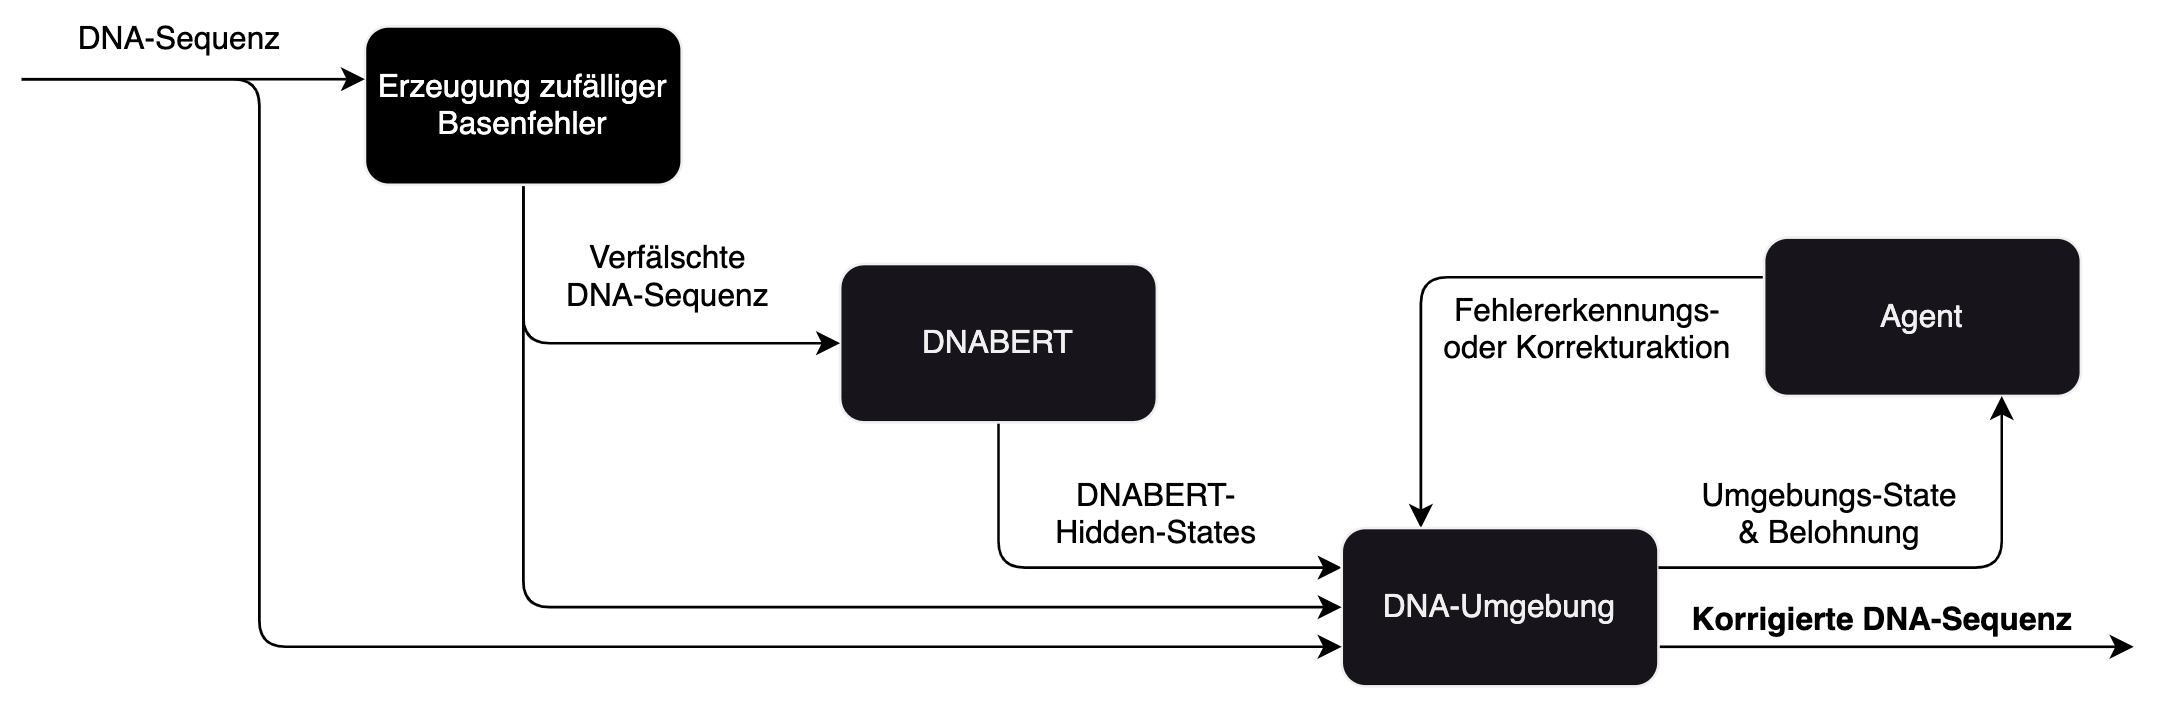
\includegraphics[width=400px,keepaspectratio]{images/Process_simplified.png}
  \caption{Vereinfachter Prozessablauf}
  \label{process_simplified}
  \end{figure}

\section{Schnittstellen}
\section{Datenmanagement}
Der Code zu dieser Arbeit 
\section{Lösungsansätze}

\section{DNA-Umgebung}

Die Aktionen des Agenten in Bezug auf das erwartete Ergebnis lassen sich unterteilen in:


\begin{itemize}
  \item True Positives: Fehlerhafte Basen der Sequenz, die erfolgreich erkannt bzw. korrigiert werden
  \item False Positives: Korrekte Basen, die fälschlicherweise als fehlerhaft erkannt werden
  \item True Negatives: Korrekte Basen, die als solche erkannt werden
  \item False Negatives: Fehlerhafte Basen, die nicht erkannt bzw. korrigiert werden
\end{itemize}
Dies wird in folgender Grafik verdeutlicht:

\begin{figure}
  \centering
  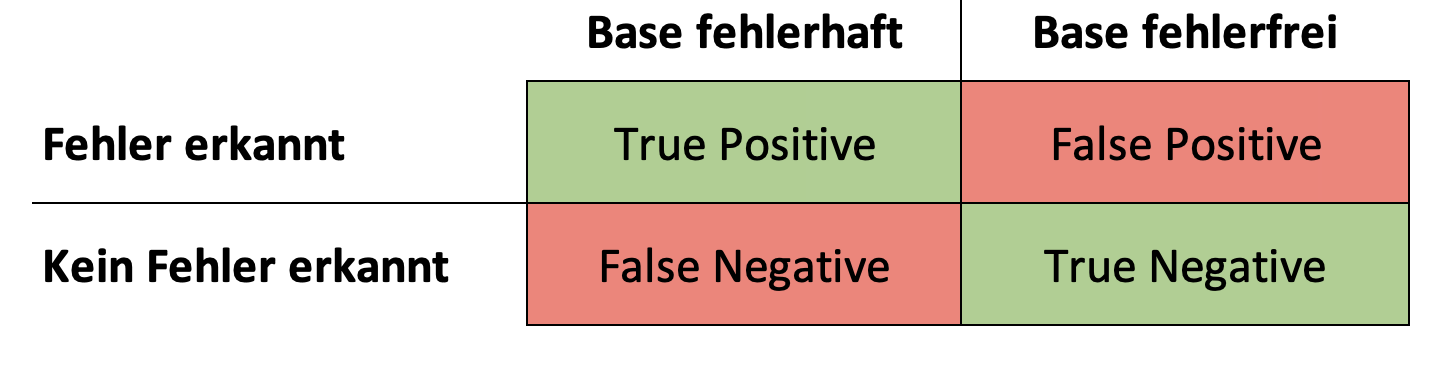
\includegraphics[width=300px,keepaspectratio]{images/TP_FN.png}
  \caption{Mögliche Entscheidungen}
  \label{TPFN}
  \end{figure}
%

\section{Erwartungswerte}

Anhand der Fehlerrate lassen sich die Erwartungswerte für eine Normalverteilung
bzw. ein untrainiertes Model berechnen. Dabei wird angenommen, dass die Action-Rate (Korrekturrate)
des Agenten gleich der Fehlerrate der DNA-Sequenz ist.

In der folgenden Grafik sind die jeweiligen Erwartungswerte für verschiedene Fehlerraten
dargestellt. Die Fehlerrate enstpricht dabei der Summe der Wahrscheinlichkeiten in der
\(Spalte\) "Base fehlerhaft". Die Action-Rate entspricht der Summe der Wahrscheinlichkeiten
in der \(Zeile\) "Fehler erkannt".

\begin{figure}
  \centering
  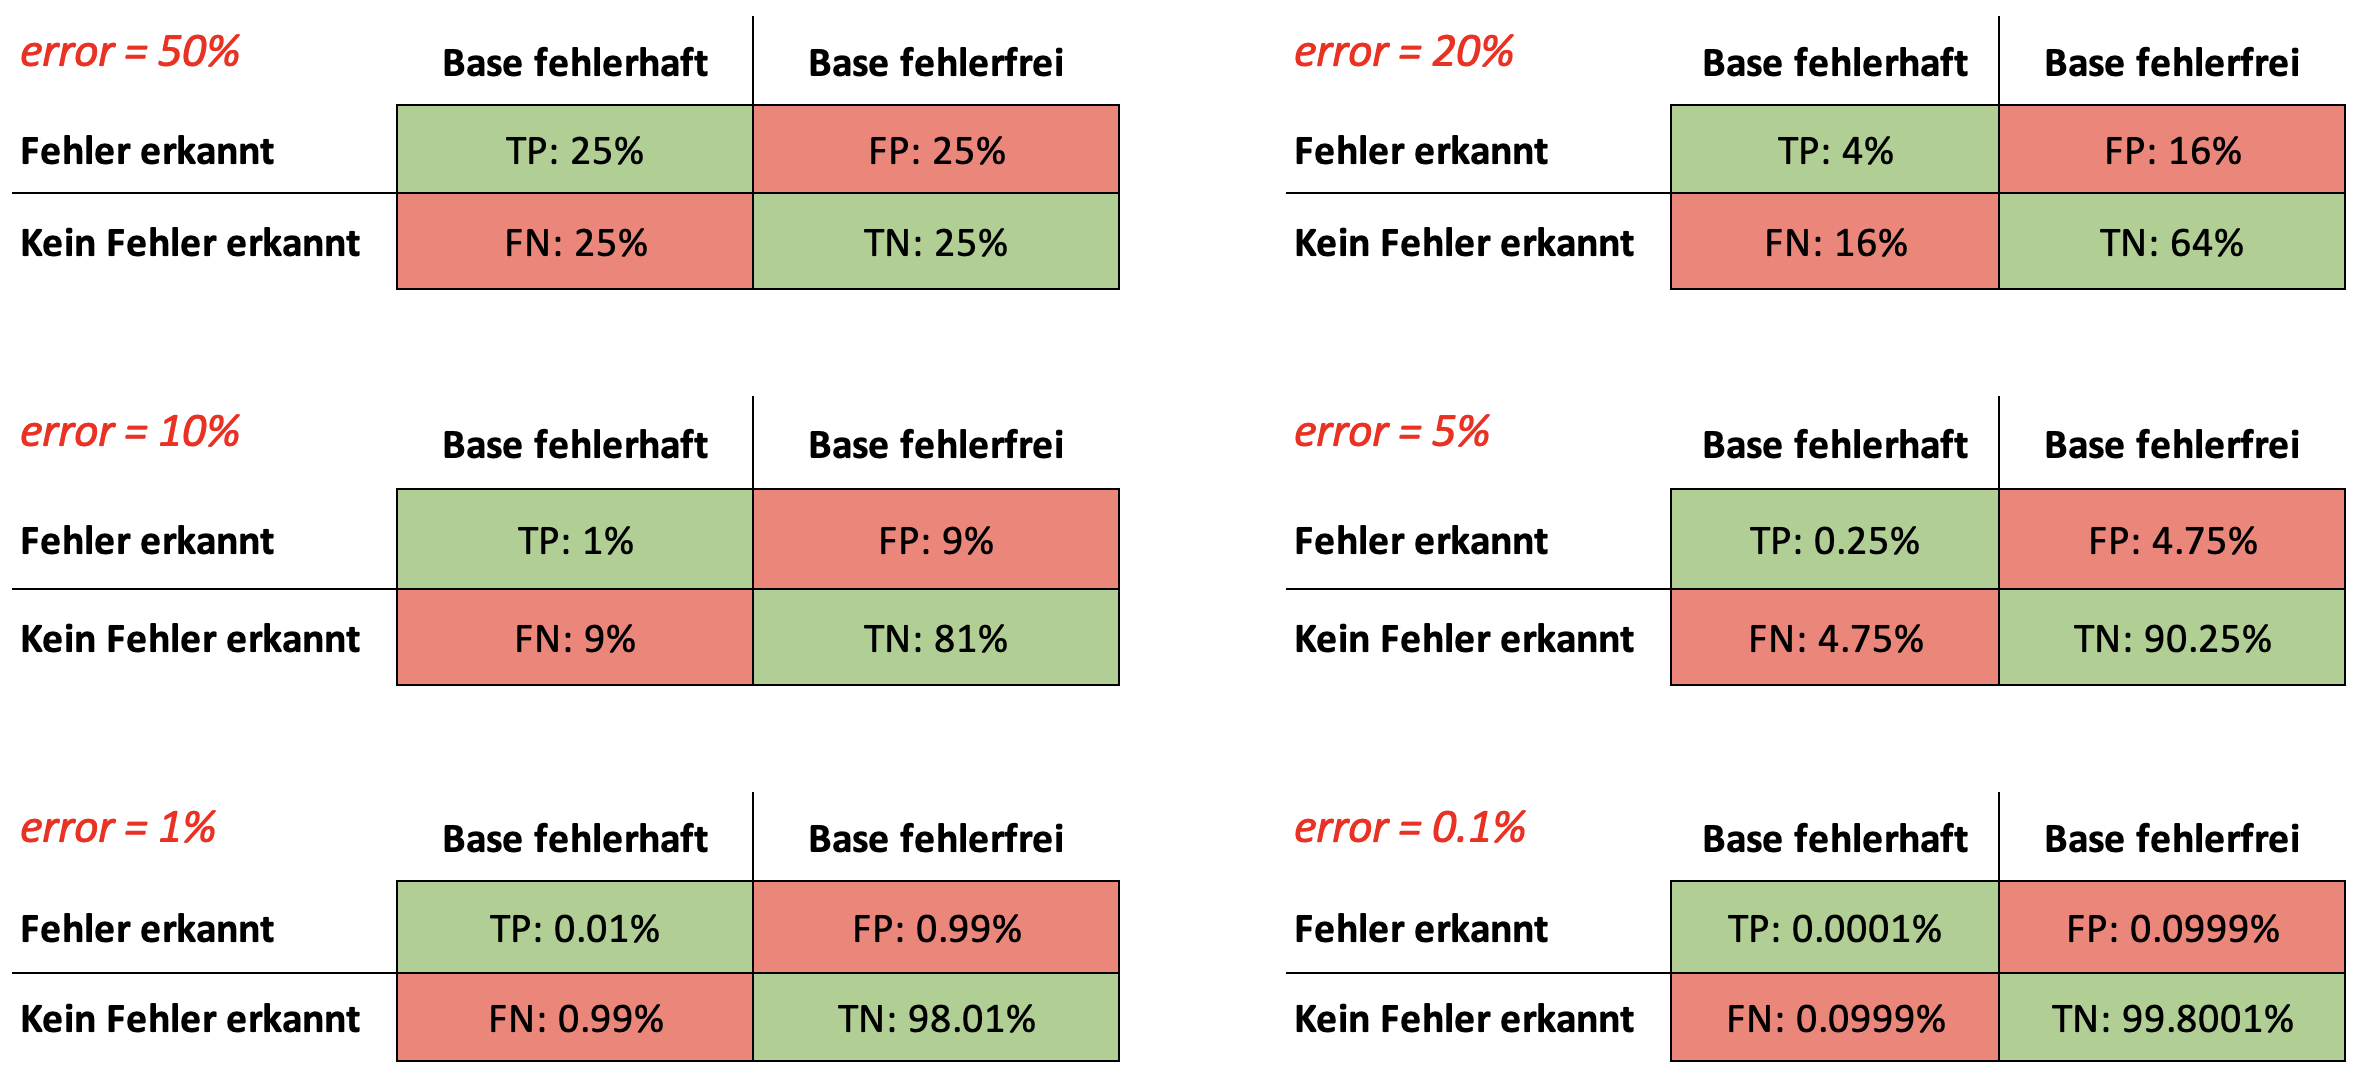
\includegraphics[width=\textwidth,keepaspectratio]{images/error_rate.png}
  \caption{Wahrscheinlichkeiten für verschiedene Fehlerraten}
  \label{probabliltiesForErrorRates}
\end{figure}


\section{Berechnung der Agenten-Belohnung}
Für die Berechnung der Belohnung des Agenten werden eine Reihe von Parametern mit einbezogen:
\begin{itemize}
  \item \(Fehlerrate\:f\): Es wird angenommen, dass die Fehlerrate unbekannt ist, bzw. nicht im Model übermittelt wird. 
Daher wird die Fehlerrate berechnet anhand der Anzahl der fehlerhaften Basen geteilt durch 
die Gesamtanzahl an verarbeiteten Basen.
\item \(Korrekturrate\:k\): Korrekturrate, also die Rate der Aktionen des Agenten bei denen eine Base als fehlerhaft markiert wird,
 wird berechnet aus der Anzahl von Korrekturaktion geteilt durch die Gesamtanzahl an verarbeiteten Basen.
 \item \(Rate\:richtiger\:Korrekturen\:k_{TP}\): Rate der richtigen Korrekturen, also der Anteil der Korrekturen, bei
 denen eine Base tatsächlich fehlerhaft war.
\end{itemize}


Anhand der Wahrscheinlichkeiten ließen sich nun statische Belohnungen für den Agenten berechnen.
Dabei geht die Summe der Belohnungen multipliziert mit den Wahrscheinlichkeiten immer gegen 0.
Beispiel für Fehlerrate = 0.1:

\begin{figure}
  \centering
  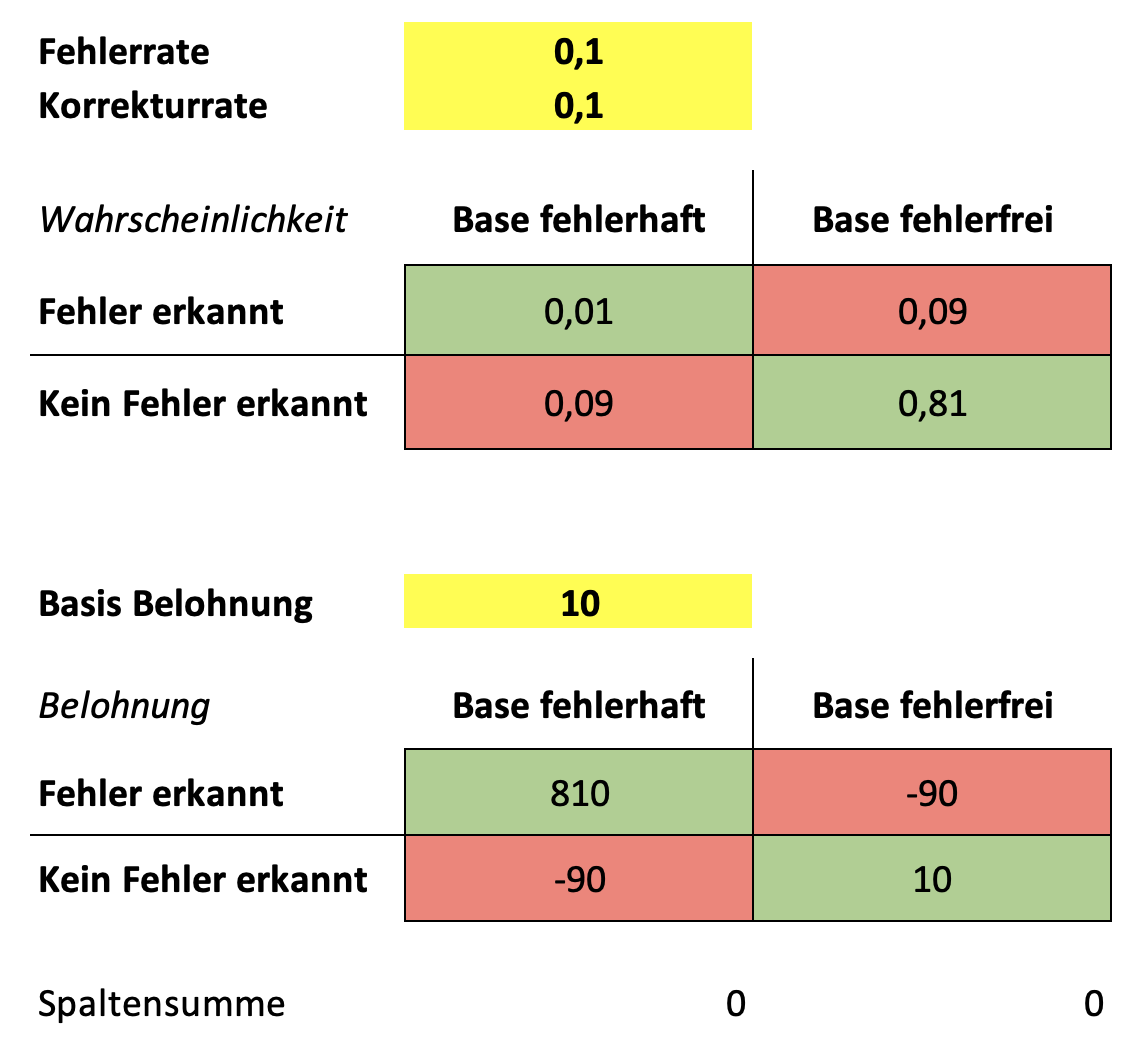
\includegraphics[width=300px,keepaspectratio]{images/static_reward.png}
  \caption{Statische Belohnung anhand der Fehlerrate}
  \label{basicRewards}
\end{figure}

Das Belohnungssystem wird so festgelegt, dass die Belohnung für True Negatives,
also Basen ohne Fehler die als korrekt erkannt wurden, immer der Basisbelohnung entspricht.
Anhand der Wahrscheinlichkeiten können dann die anderen Belohnungen berechnet werden:
\linebreak[4]

\begin{figure}
\begin{align*}
  B &= 10 \\
  B_{TN} &= B & = 10 \\
  B_{FN} &= - B * P_{TN} / P_{FN} \\
  &= -10 * 0.81 / 0.09 &= -90 \notag\\
  B_{FP} &= - B * P_{TN} / P_{FP} \\
  &= -10 * 0.81 / 0.09 &= -90 \notag\\
  B_{TP} &= B * P_{TN} / P_{TP} \\
  &= 10 * 0.81 / 0.01 &= 810 \notag\\
\end{align*} 


\begin{conditions}
  B & Basisbelohnung \\
  B_{TN} & Belohnung für True Negatives \\
  B_{TP} & Belohnung für True Positives \\
  B_{FN} & Belohnung für False Negatives \\
  B_{FP} & Belohnung für False Positives \\
  P_{TN} & Wahrscheinlichkeit für True Negatives \\
  P_{TP} & Wahrscheinlichkeit für True Positives \\
  P_{FN} & Wahrscheinlichkeit für False Negatives \\
  P_{FP} & Wahrscheinlichkeit für False Positives
\end{conditions}

\end{figure}
\leavevmode \\


Optimierung 1:
Das Belohnungssystem soll so gebaut werden, dass die Summe der Belohnungen für eine Spalte der Tabelle
im Durchschnitt 0 ergeben. Dafür müssen die Belohnungen mit der Zeit angepast werden, abhängig von der
Performance des Agenten. Wenn der Agent mit der Zeit besser darin wird 
Allerdings ist an den Wahrscheinlichkeiten auch erkenntlich, 
dass mit abnehmender Fehlerrate die Wahrscheinlichkeit für ein True Positive schnell sehr klein wird.
Sie entspricht der Fehlerrate multipliziert mit der Korrekturrate.
Da angenommen wurde, dass die Korrekturrate gleich der Fehlerrate ist, ist die Wahrscheinlichkeit
für ein True Positive die Fehlerrate zum Quadrat \(P_{TP} = f^2\). 

Eine so geringe Wahrscheinlichkeit für ein Erfolgserlebnis des Agenten könnte den Lernprozess deutlich verlängern.
Dabei ist die Annahme, dass die Korrekturrate der Fehlerrate entspricht nur eine Idealvorstellung, die erst wirklich sinnvoll
ist sobald der Agent alle bzw. einen Großteil der Fehler erkennt und dabei keine neuen produziert.
Für ein untrainiertes Model ist es sinnvoller, dass die Korrekturrate deutlich über Fehlerrate liegt. 
Dadurch werden zwar mehr neue Fehler verursacht, allerdings wird auch ein größerer Anteil der ursprünglichen Fehler
gefunden. Der Agent wird somit experimentierfreudiger bei seinen Korrekturen.

Jedoch ist die Korrekturrate kein Parameter, welcher dem Model übermittelt wird.
Sie wird vom Agenten selbst festgelegt, anhand der Belohnungen. 
Ein möglicher Ansatz, die Korrekturrate des Agenten zu erhöhen, ist eine stärkere Gewichtung der Belohnungen für die Spalte "Base fehlerhaft".
Der Agent soll mehr Fehler finden, auch wenn dabei mehr neue Fehler produziert werden.
Er muss also noch höhere Belohnungen kriegen, wenn ein Fehler gefunden wurde,
und mehr Abzug wenn ein Fehler übersehen wurde. Die Summe der Belohnungen der Spalte 
multipliziert mit den Wahrscheinlichkeiten sollte jedoch weiterhin 0 ergeben.
Um die Belohnungen der Spalte für fehlerhafte Basen stärker zu gewichten, wird zunächst eine
gewünschte Korrekturrate berechnet anhand der aktuellen Performance des Models berechnet.
Um die Performance zu beurteilen, wird geschaut wie groß der Anteil der richtigen Korrekturen
an der Gesamtanzahl der Korrekturen ist. Nachdem die gewünschte Korrekturrate berechnet wurde,
wird anhand dessen und anhand der tatsächlichen Korrekturrate ein Gewichtungsfaktor g berechnet.
Bei einer Normalverteilung wie in Darstellung \ref{probabliltiesForErrorRates} sollte die gewünschte 
Korrekturrate etwa 50\% betragen und mit besserer Performance des Models langsam abnehmen. 
Mit nahezu perfekter Performance, also eine Erkennung aller Fehler ohne neue Fehler zu produzieren,
sollte sich die Korrekturrate der Fehlerrate angleichen.

\begin{figure}
  \begin{align*}
    k_{TP} &= c_{TP} / c_{P} \\
    k_{desired} &= 0.1 + (1 - k_{TP} ) / 2 \\
    g &= k_{desired} / k_{actual}
  \end{align*} 
  
  \begin{conditions}
    k_{TP}      & Anteil der richtigen Korrekturen (True Positives) \\
                & an der Gesamtkorrekturzahl \\
    c_{TP}      & Anzahl der richtigen Korrekturen (True Positives) \\
    c_{P}       & Anzahl der gesamten Korrekturen (Positives) \\
    k_{desired} & Gewünschte Korrekturrate \\
    k_{actual}  & Tatsächliche Korrekturrate \\
    g           & Gewichtungsfaktor der Belohnungen für fehlerhafte Basen
  \end{conditions}
  
  \end{figure}
  \leavevmode \\

Die Belohnungen für fehlerhafte Basen werden mit dem Gewichtungsfaktor g multipliziert.



\subsection{Basenweise Verarbeitung}
Bei der basenweisen Verarbeitung der DNA-Sequenz wird jede Base, zusammen mit ihrem zugehörigen BERT-Vektor, 
einzeln in das Model gefüttert.
Der aktuelle State des Agenten entspricht dabei immer dem BERT-Vektor der aktuell zu korrigierenden Base. 
Auf diese Weise wird der State kleingehalten. Ist der State des Agenten zu groß, kann es schwierig werden, 
den Agenten erfolgreich zu trainieren. Ein großer State erfordert mehr Speicher und Rechenleistung, 
um den State zu verarbeiten und eine Aktion auszuwählen. 
Es kann auch schwieriger werden, eine geeignete Belohnungsfunktion zu definieren, 
da es schwieriger sein kann, die Auswirkungen der Aktionen des Agenten auf den State zu verstehen.


\subsubsection{Fehlererkennung}
Um den Lernprozess des RL-Models zu vereinfachen, wurde es zunächst darauf trainiert die Fehler nur zu erkennen, statt sie zu korriegen.
Die Action-Space wird dadurch auf zwei Aktionen reduziert: Base als korrekt (0) und als fehlerhaft markieren (1).
Dadurch soll der Agent für jede Sequenz eine Fehlerkarte erstellen. 
Damit ist ein Array gemeint, welcher den Wert 1 an jeder Position einer fehlerhaften Base enthält und den Wert 0 an den Positionen aller korrekten Basen.

\subsubsection{Fehlerkorrektur}
Bei der Fehlerkorrektur soll ein Fehler in einer DNA-Sequenz nicht nur erkannt werden, sonden auch durch die richtige Base ersetzt werden.
Dabei gibt es zwei mögliche Ansätze: 
Die erste Möglichkeit ist, dass der Agent selber eine Entscheidung über die Auswahl der richtigen Base trifft. 
In diesem Fall müsste der Agent aus vier Aktionen auswählen können, da es vier Basen gibt. 
Der Korrekturprozess müsste von grundauf erlernt werden.
Die zweite Möglichkeit ist, dass der Agent die falschen Basen weiterhin nur als fehlerhaft markiert
und anschließend für das DNABERT-Model maskiert. 
Danach wird die Sequenz erneut von DNABERT verarbeitet
und neue Hidden-States werden generiert. Der Agent hat dann die Möglichkeit,
die Base erneut anhand des neuen DNABERT-States zu beurteilen. 
Die tatsächliche Korrektur einer Base findet somit im DNABERT-Model statt, da fehlerhafte
Basen einfach als maskiert behandelt werden.

\subsubsection{1. Ansatz: Korrektur durch Agent}
Soll die Korrektur rein beim Agenten erfolgen, so muss der Agent nicht nur aus zwei Aktionen 
auswählen können (Fehler / kein Fehler) sondern aus mindestens vier Aktionen. 
Für die Auswahl dieser vier Aktionen gibt es zwei verschiedene Ansätze:
1. Die Aktionen können direkt für eine bestimmte DNA-Base stehen:

\begin{itemize}
  \item Aktion 1: A
  \item Aktion 2: T
  \item Aktion 3: G
  \item Aktion 4: C
\end{itemize}

Dadurch muss der Agent in jedem Fall die richtige Base vorhersagen, auch wenn die Base fehlerfrei ist.
Er kann nicht auf eine Standardaktion für fehlerfreie Basen zurückgreifen, sondern muss immer individuell entscheiden.
Das kann sowohl als Vorteil und Nachteil angesehen werden: 
Der Agent lernt, zusätzlich dazu fehlerhafte Basen zu korrigieren,
auch fehlerfreie BERT-Vektoren den richtigen Basen zuzuordnen.
Die Aufgabe wird dadurch komplexer, was die Trainingszeit verlängern könnte, allerdings könnten die Korrekturentscheidungen
am Ende des Trainings auch genauer sein, da ein tieferes Verständnis von den DNA-Fehlern bzw. deren Encoding in BERT-Hidden-States erlangt wurde.

2. Eine andere Möglichkeit ist, die Aktion auf eine Verschiebung der Basen zu beziehen. 
Damit ist eine Verschiebung des Indexes der Base gemeint, in einer Liste aller Basen:

Index: [0, 1, 2, 3]
Basen: [A, T, G, C]

Jeder Base wird ein Index zugewiesen. Die Aktion des Agenten entspricht der Anzahl an Schritten, die auf den aktuellen Basenindex
addiert werden. Wird der Index zu weit nach rechts verschoben, so wird zurückgesprungen zum Index 0. 
Dafür wird der Modulo der Indexsumme (Aktueller Index + Verschiebung) gezogen:\\

\begin{figure}
\begin{align*}
i_{new} = (i + s)\mod 4\\
\end{align*}
\begin{conditions}
  i      & Index \\
  i_new  & Neuer Index nach der Basenverschiebung \\
  s      & Verschiebungszahl \\
\end{conditions}
\end{figure}

\begin{itemize}
  \item Aktion 0: Keine Verschiebung
  \item Aktion 1: Indexverschiebung um 1
  \item Aktion 2: Indexverschiebung um 2
  \item Aktion 3: Indexverschiebung um 3
\end{itemize}

Fehlerfreie Basen werden dadurch immer mit der gleichen Aktion behandelt (Aktion 0). 


\subsubsection{2. Ansatz: Korrektur durch DNABERT Maskierung}
Ein einfacherer Ansatz, fehlerhafte Basen zu korrigieren, ist die Nutzung der
Basenmaskierung, auf die das DNABERT-Model bereits trainiert wurde. 
Dabei wird jede Base, die vom Agenten als fehlerhaft erkannt wird, 
maskiert und erneut vom DNABERT-Model verarbeitet.
Was das Training des Agenten betrifft sollte dieser Ansatz deutlich simpler sein,
da der Agent nicht die Korrektur, also die Auswahl der richtigen Base, übernehmen muss.
Er muss die Fehler weiterhin nur erkennen und zusätzlich den neuen, 
anhand der maskierten Base generierten DNABERT-State beurteilen.

Die Aktionen werden dabei erweitert, sodass der Agent auch einen Schritt zurück in der Sequenz gehen kann.
Dadurch können vorherige Entscheidungen erneut beurteilt werden.

\begin{itemize}
  \item Aktion 0: Schritt zurück, keine Korrektur der aktuellen Base (Index - 1)
  \item Aktion 1: Schritt vor, keine Korrektur der aktuellen Base  (Index + 1)
  \item Aktion 2: Maskierung der aktuellen Base, Berechnung der neuen DNABERT-States, Index bleibt gleich
\end{itemize}



\subsection{Sequenzweise Verarbeitung}
\subsubsection{Fehlererkennung}
\subsubsection{Fehlerkorrektur}
\section{...}


\clearpage


\chapter{Implementierung}

\section{OpenAI Gym-Environments}

Für die Umsetzung der verschiedenen DNA-Korrekturansätze wurden Gym-Environments genutzt.
Gym-Environments sind simulierte Umgebungen, die zum Training von KI-Agenten verwendet werden. 
Diese Umgebungen stellen dem Agenten eine Reihe von Beobachtungen, Aktionen und Belohnungen zur Verfügung, 
und das Ziel des Agenten ist es, eine Politik zu lernen, 
die die erwartete kumulative Belohnung im Laufe der Zeit maximiert. 
Die Umgebung kann einfach sein, wie z.B. ein Spiel, bei dem der Agent einen einzelnen Charakter steuert und 
ein Ziel erreichen muss, oder sie kann komplex sein, wie z.B. eine realistische Simulation eines Autos, 
das in einer Stadt fährt. 
Gym-Umgebungen werden oft verwendet, um Reinforcement-Learning-Agenten zu trainieren, 
können aber auch verwendet werden, um andere Arten von Agenten zu trainieren, 
wie z.B. supervised Learning und unsupervised Learning Agenten.

%Gym übernimmt die Modelierung einer Umgebung, in der ein Reinforcement Learing Agent trainiert werden kann.
Um ein Gym-Environment zu erstellen, muss eine Klasse erstellt werden, 
die von gym.Env erbt und folgende Methoden implementiert:

- def step(action)
- def reset()

Die step-Methode führt eine einzige Aktion durch auf dem aktuellen State durch, wodurch ein neuer State entsteht.
Anschließend wird für die durchgeführte Aktion ein Reward berechnet. Der Reward wird zusammen mit dem neuen State zurückgegeben. 
Außerdem wird ein "done"-Boolean Flag zurückgegeben, welches anzeigt ob die aktuelle Runde beendet ist.

Die Reset-Methode wird ausgeführt, wenn die aktuelle Runde beendet wurde. 
Also immer dann, wenn die Step-Methode den Wert True für das done-Flag zurückgibt. 
Reset setzt die Umgebung in einen Ausgangszustand zurück, indem ein initialer State gesetzt wird auf dem noch keine Aktion erfolgt ist.

\section{Umsetzung der Ansätze}

Um die verschiedenen Ansätze der Fehlererkennung und -korrektur zu implementieren, werden die Umgebungen folgendermaßen unterteilt:

\begin{itemize}

  \item \textbf{1. Nukleotid-weise Verarbeitung:} Hierbei wird die DNA-Sequenz Base für Base verarbeitet. Der State des Agenten ist dabei die DNABERT-Kodierung
  der aktuellen Base für jeden Korrekturschritt. 

  \begin{itemize}

    \item \textbf{1.1. Ein Durchlauf mit mehreren Korrekturen:} In diesem Ansatz wird die Sequenz nur einmal verarbeitet und es wird probiert, alle Fehler 
    in nur einem Durchgang zu erkennen. Die Runde ist abgeschlossen, wenn das Ende der Sequenz erreicht ist.
    Dabei sind die Aktionen des Agenten: Die Fehlererkennung/-korrektur der aktuellen Base und einen Schritt vorwärts in der Sequenz zu gehen.
    Zusätzlich könnte eine weitere Aktion, für einen Schritt zurück in der Sequenz, eingebaut werden. Dies würde dem Agenten die Chance geben,
    eine bereits korrigierte Base erneut auf Richtigkeit zu prüfen. Die Entscheidung könnte beim nächsten Versuch anders ausfallen, 
    wenn der Agent bereits mehr Basen der Sequenz verarbeitet hat.

    \begin{itemize}

      \item \textbf{1.1.1. Fehlererkennung:} Bei der Fehlererkennung muss der Agent sich nicht für eine korrigierte Base entscheiden. Er muss die Fehler 
      nur erkennen, also jede Base als fehlerfrei (0) oder fehlerhaft (1) kennzeichnen.

      \item \textbf{1.1.2. Fehlerkorrektur:} Hier muss der Agent im Falle einer Fehlererkennung auch die richtige Base auswählen, um den Fehler zu korrigieren.
      Die Erfolgschance, also die Chance auf die richtige Korrektur einer tatsächlich fehlerhaften Base, ist hierbei nur noch ein Drittel
      der Chance zur Fehlererkennung, da der Agent aus drei möglichen Korrekturbasen entscheiden muss. Die Belohnung für einen Erfolg
      wurde daher verdreifacht.

      \item \textbf{1.1.3. Fehlererkennung mit DNABERT-Maskierung:} Dies ist eine Erweiterung der Fehlererkennung, wo die Korrektur einer fehlerhaften Base 
      nicht vom Agenten übernommen wird, sondern vom DNABERT-Modell. Dafür wird die Maskierungsfunktion des DNABERT genutzt. 
      Wenn der Agent eine Fehler erkennt, werden die DNABERT-Hidden-States erneut für die Sequenz generiert, wobei die fehlerhafte Base
      maskiert wird. Dabei entsteht ein neuer State für diese Base. 
      Außerdem wird die Umgebung so angepasst, dass im Falle einer Fehlererkennung kein Schritt vorwärts gemacht wird. 
      Stattdessen bleibt die Position gleich und der vorherige State der maskierten Base wird gespeichert. 
      Wenn der Agent in der nächsten Iteration die gleiche Position erneut als fehlerhaft erkennt, wird die Maskierung wieder
      zurückgesetzt und der alte, zwischengespeicherte State der Base wird wieder an der Stelle eingesetzt.
      Dadurch bekommt der Agent die Möglichkeit, eine als fehlerhaft erkannte Base erneut zu beurteilen, nachdem DNABERT einen
      Korrekturvorschlag erzeugt hat. 
      Die Anzahl an Schritten pro Sequenz ist damit von Aktionen des Agenten abhängig, also wurde das Belohnungssystem so erweitert,
      das jeder Korrektureingriff pauschal eine Belohnung von minus eins gibt. 
      Die tatsächliche Belohnung für die Korrektur oder Verfälschung einer Base bekommt der Agent erst, wenn er mit der Base abschließt, 
      also einen Schritt vorwärts in der Sequenz geht.
      
    \end{itemize}

    \item \textbf{1.2. Mehrere Durchläufe mit jeweils einer Korrektur:} Im gegensatz zum Ansatz 1.1., werden hier mehrere Durchläufe pro Sequenz gemacht,
    wobei in jedem Durchlauf nur ein einziger Korrektureingriff gemacht wird. Da die Sequenz auch hier Base für Base verarbeitet wird,
    und der Agent nach jeder Base eine Aktion trifft, muss der Korrektureingriff erst am Ende der Sequenz erfolgen. 
    Dafür wird kein diskreter Action-Space mehr genutzt, sondern ein Box-Space. Die Aktion ist somit ein Wert zwischen null und eins
    und kann somit als Wahrscheinlichkeit interpretiert werden. Der Agent trifft für jede Base eine Korrekturwahrscheinlichkeit
    und entscheidet sich am Ende für eine Korrektur der Base mit der höchsten Wahrscheinlichkeit.
    Schwierig ist hierbei die Entscheidung, wann der Agent mit der Korrektur einer Sequenz aufhören soll, da das Ende der Sequenz als Kriterium
    nicht mehr gültig ist, wenn mehrere Durchläufe stattfinden.
    
    \begin{itemize}
    
      \item \textbf{1.2.1. Fehlererkennung:} Siehe 1.1.1.
    
      \item \textbf{1.2.2. Fehlerkorrektur:} Für die Korrektur müsste jede Aktion des Agenten zusätzlich zur Wahrscheinlichkeit, auch einen diskreten
      Wert für die Auswahl der Korrekturbase enthalten. Der Action-Space müsste also einen Box-Space und einen Discrete-Space enthalten.
      Dieser Ansatz wurde nicht weiter verfolgt, nachdem die Erfolgsrate für 1.2.1. sehr gering war.
      
    \end{itemize}

  \end{itemize}

  \item \textbf{2. Sequentielle Verarbeitung:} Bei der Sequenziellen Verarbeitung sieht der Agent in jedem Schritt die ganze Sequenz. Der State entspricht 
  nicht nur DNABERT-State einer Base, sondern einem Array aller DNABERT-States, und wird damit sehr groß.
  Der Agent kann entweder mehrere Korrekturen pro Durchgang vornehmen, oder nur einen einzigen.
  In jedem Fall wird die Sequenz mehrfach verarbeitet, daher ist es auch hier schwierig zu entscheiden, wann die Korrektur einer Sequenz beendet ist.
  
  \begin{itemize}

    \item \textbf{2.1 Fehlererkennung mit DNABERT-Maskierung:} DNABERT wird für die Fehlerkorrektur genutzt. Gerade hier macht es Sinn, dass 
    der Agent die Sequenz mehrfach verarbeitet und somit maskierte Basen erneut berurteilen kann.
    
    \item \textbf{2.1 Fehlerkorrektur:} Agent korrigiert Basen eigenständig. Wurde nicht umgesetzt aufgrund von geringem Erfolg mit 2.1.
    
  \end{itemize}

\end{itemize}

\clearpage

Um die genauen Unterschiede zwischen den Ansätzen klar hervorzubringen, wurden die Umgebungen durch eine Vererbungshierarchie umgesetzt:

\begin{figure}[t!]
  \centering
  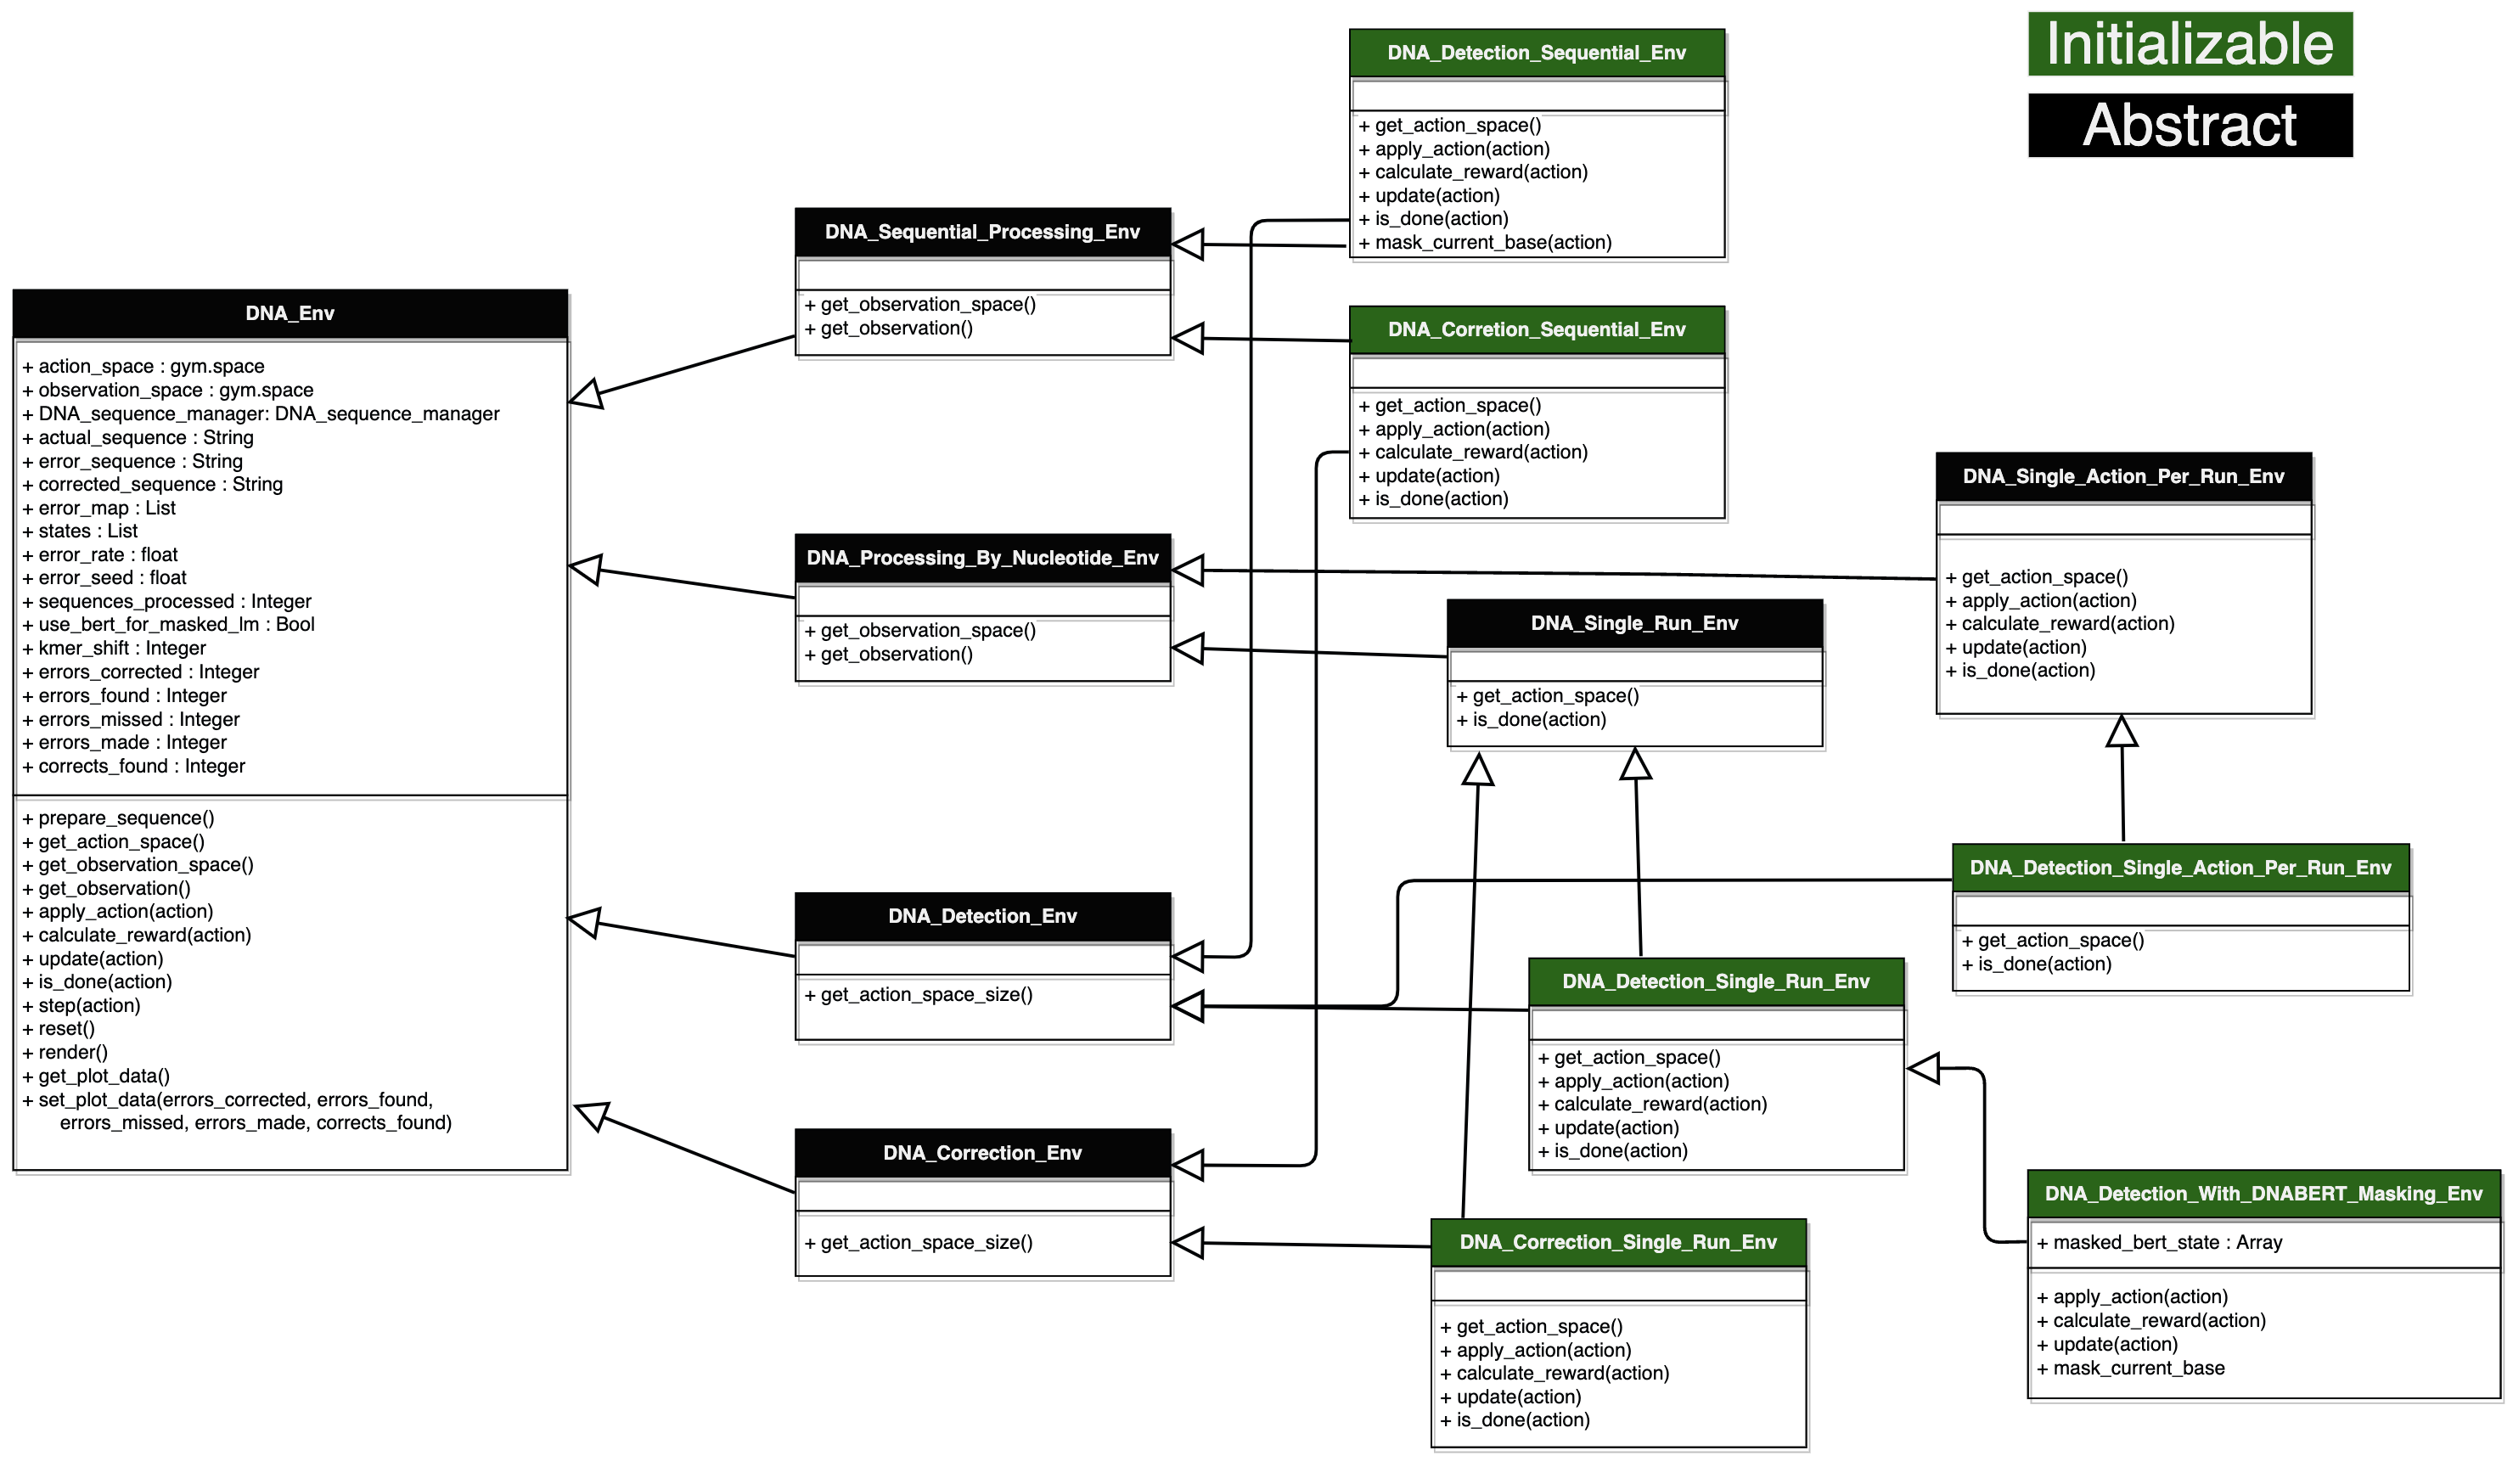
\includegraphics[width=400px,keepaspectratio]{images/classes.png}
  \caption{Implementierung der Gym-Environments}
  \label{gymClasses}
\end{figure}

\begin{lstlisting}[caption={Ein Beispiel: Hello World (Scala)}]
object HelloWorld {
  def main(args: Array[String]): Unit = {
    println("Hello, world!")
  }
}
\end{lstlisting}

Umfangreicher Quell-Code sollte in den Anhang ausgelagert werden.]


\chapter{Test}
TODO / TBD

\chapter{Darstellung und Bewertung der Ergebnisse}
[Beschreibung der Ergebnisse aus allen voran gegangenen Kapiteln sowie der zuvor generierten Ergebnisartefakte mit Bewertung, wie diese einzuordnen sind]

\chapter{Beurteilung des Reinforcement Learning als Ansatz zur DNA-Fehlerkorrektur}
Durch die Umsetzung des Reinforcement-Learning-Ansatzes zur DNA-Fehlerkorrektur wurden wichtige Erkenntnisse erlangt,
vorallem in Bezug auf die Eignung von Reinforcement-Learning als Tool für die Korrektur von sequentiellen Daten.
Aus den Testergebnissen geht hervor, dass der Ansatz zumindest zu Teilen funktioniert und der
Agent lernt die DNABERT-States als fehlerhaft oder fehlerfrei zu klassifizieren, wenn auch sehr langsam.
In der Praxis könnte dieses Model mit dem aktuellen Trainingsstand allerdings niemals eingesetzt werden, 
da jedes der Modelle noch deutlich mehr Fehler in korrekten Basen produziert, als das fehlerhafte Basen erkannt werden.

Aufgrund der langen Trainingszeiten mit mittelmäßigen Resultaten und der allgemeinen Theorie hinter Reinforcement Learning,
sollte dieser Ansatz nochmal hinterfragt werden. 
Reinforcement Learning ist ein hervorragendes Tool für Problemumgebungen mit imperfektem Informationsgehalt.
Dazu zählen zum Beispiel die meisten Kartenspiele wie Poker, wo man nur die eigenen Karten kennt, oder die 
Steuerung von Robotern oder Spielecharakteren in unbekannten Umgebungen.
Die Korrektur von Fehlern in DNA-Sequenzen ist jedoch ein Problem mit perfektem Informationsgehalt, da beim Training
die jeweils richtige Base für jede fehlerhafte Base der Sequenz bekannt ist.
Die Information, ob die ursprüngliche Base fehlerhaft war oder nicht, wird dafür verwendet die Agenten-Belohnung 
zu berechnen.

Stattdessen könnte diese Information auch der Ziel-Output von einem anderem Machine Learning Modell sein, welches direkt
auf einen bestimmten Output trainiert wird, anstatt Aktionen auszuprobieren und dafür Belohnt zu werden.
 
Zum Vergleich wurde Versucht, ein eindimensionales CNN auf die Erkennung der Sequenzierungsfehler zu trainieren.


\chapter{Zusammenfassung}
TODO / TBD
[Aggregierte retrograde Kurzbeschreibung der Arbeit]
\section{Schlussfolgerungen}
TODO / TBD
[Beschreibung der insgesamt zu konstatierenden Schlussfolgerungen im Zusammenhang mit der Arbeit]
\section{Limitationen}
TODO / TBD
[Beschreibung der Ergebnisse einer kritischen Reflektion und Begründung dessen, was die Arbeit nicht zu leisten vermag]
\section{Ausblick}
TODO / TBD
[Beschreibung und Begründung potenzieller zukünftiger Folgeaktivitäten im Zusammenhang mit Ihrer Arbeit (z.B. weitere Anforderungen, Theoriebildung, ... ]


















%\bibliographystyle{plain}
%\bibliography{bibliography}





%----------------------------------------------------------------------------------------
%	REFERENCE LIST
%----------------------------------------------------------------------------------------


% \bibliographystyle{apalike}
% \bibliographystyle{ksfh_nat} % ein anderer Stil
% \bibliography{science} 

\begin{thebibliography}{XX}
\bibitem[]{transformer}T. Bielecki, M. Rutkowski, Credit Risk: Modeling, Valuation and Hedging, Springer (2002).

%\bibitem[Bielecki, Rutkowski(2002)]{bielecki02}T. Bielecki, M. Rutkowski, Credit Risk: Modeling, Valuation and Hedging, Springer (2002).
%\bibitem[Jarrow, Turnbull(1995)]{jarrow95} R.A. Jarrow, S. Turnbull, Pricing derivatives on financial securities subject to credit risk, Journal of Finance, 50:1 (1995) 53--85.
%\bibitem[Marshall, Olkin(1967)]{marshall67} A.W. Marshall, I. Olkin, A multivariate exponential distribution, Journal of the American Statistical Association, 62 (1967), pp. 30--44.
%\bibitem[Schönbucher(2003)]{schoenbucher03} P.J. Schönbucher, Credit Derivatives Pricing Models, Wiley (2003).
\end{thebibliography}

\printbibliography[
heading=bibintoc,
title={Quellenverzeichnis}
]


\newpage

\chapter{Abkürzungsverzeichnis}
\newpage
\chapter{Glossar}




\begin{appendix}

\pagenumbering{Roman}

\chapter{Appendix}


\section{Quell-Code}

\section{Tipps zum Schreiben Ihrer Abschlussarbeit}

\begin{itemize}
\item Achten Sie auf eine neutrale, fachliche Sprache. Keine \glqq{}Ich\grqq{}-Form.
%\item Zitieren Sie zitierfähige und -würdige Quellen (z.B. wissenschaftliche Artikel und Fachbücher; nach Möglichkeit keine Blogs und keinesfalls Wikipedia\footnote{Wikipedia selbst empfiehlt, von der Zitation von Wikipedia-Inhalten im akademischen Umfeld Abstand zu nehmen \autocite{wikipedia2019}.}). 
\item Zitieren Sie korrekt und homogen.
\item Verwenden Sie keine Fu{\ss}noten für die Literaturangaben.
\item Recherchieren Sie ausführlich den Stand der Wissenschaft und Technik.
\item Achten Sie auf die Qualität der Ausarbeitung (z.B. auf Rechtschreibung).
\item Informieren Sie sich ggf. vorab darüber, wie man wissenschaftlich arbeitet bzw. schreibt:
\begin{itemize}
%\item Mittels Fachliteratur\footnote{Z.B. \autocite{balzert2011}, \autocite{franck2013}}, oder
\item Beim Lernzentrum\footnote{Weitere Informationen zum Schreibcoaching finden sich hier: \url{https://www.htw-berlin.de/studium/lernzentrum/studierende/schreibcoaching/}; letzter Zugriff: 13 VI 19.}.
\end{itemize}
\item Nutzen Sie \LaTeX\footnote{Kein Support bei Installation, Nutzung und Anpassung allfälliger \LaTeX-Templates!}.
\end{itemize}



\newpage
% Letzte Seite
\thispagestyle{empty}       % keine Seitennummer
%\vspace*{18cm}
\noindent

\section*{Eidesstattliche Versicherung}
Hiermit versichere ich an Eides statt durch meine Unterschrift, dass ich die vorstehende Arbeit selbstständig und ohne fremde Hilfe angefertigt und alle Stellen, die ich wörtlich oder annähernd wörtlich aus Veröffentlichungen entnommen habe, als solche kenntlich gemacht habe, mich auch keiner anderen als der angegebenen Literatur oder sonstiger Hilfsmittel bedient habe. Die Arbeit hat in dieser oder ähnlicher Form noch keiner anderen Prüfungsbehörde vorgelegen.\\
\linebreak[4]
\linebreak[4]
\linebreak[4]
\linebreak[4]
-------------------------------------------------------\linebreak[4]
Datum, Ort, Unterschrift


\end{appendix}


\end{document}

